\documentclass{report}

\usepackage{graphicx}
\graphicspath{{./Set/images/}}

\usepackage{amsfonts, amsmath, amssymb, amsthm}
\usepackage{bigfoot}
\usepackage{comment}
\usepackage[shortlabels]{enumitem}
\usepackage{etoolbox}
\usepackage{environ}
\usepackage{fontawesome5}
\usepackage{mathabx, mathrsfs}
\usepackage{soul}
\usepackage{stmaryrd}
% Must load `xcolor` before `tcolorbox` and `tikz`.
\usepackage[dvipsnames]{xcolor}
\usepackage{tcolorbox}
\usepackage{tikz}
% `hyperref` comes after `xr-hyper`.
\usepackage{xr-hyper}
\usepackage{hyperref}

% Open "private" namespace.
\makeatletter

% ========================================
% General
% ========================================

\newcommand{\header}[2]{\title{#1}\author{#2}\date{}\maketitle}

% ========================================
% Dividers
% ========================================

\newcommand\@linespace{\vspace{10pt}}
\newcommand\linedivider{\@linespace\hrule\@linespace}
\WithSuffix\newcommand\linedivider*{\@linespace\hrule}
\newcommand\suitdivider{$$\spadesuit\;\spadesuit\;\spadesuit$$}

% ========================================
% Linking
% ========================================

\hypersetup{colorlinks=true, linkcolor=blue, urlcolor=blue}
\newcommand{\textref}[1]{\text{\nameref{#1}}}
\newcommand{\hyperlabel}[1]{%
  \label{#1}%
  \hypertarget{#1}{}}

% Links to theorems/statements/etc. that can be found in Mathlib4's index.
\newcommand\@leanlink[3]{%
  \textcolor{BlueViolet}{\raisebox{-4.5pt}{%
    \tikz{\draw (0, 0) node[yscale=-1,xscale=1] {\faFont};}}{-\;}}%
  \href{https://leanprover-community.github.io/mathlib4_docs/#1.html\##2}%
  {\color{BlueViolet}{#3}}}

\newcommand\lean[2]{%
  \noindent\@leanlink{#1}{#2}{#2}}
\WithSuffix\newcommand\lean*[2]{%
  \vspace{6pt}\lean{#1}{#2}}

\newcommand\leanp[3]{%
  \noindent\@leanlink{#1}{#2}{#3}}
\WithSuffix\newcommand\leanp*[3]{%
  \vspace{6pt}\leanp{#1}{#2}{#3}}

% Links to theorems/statements/etc. found in custom index.
\newcommand\@codelink[4]{%
  \textcolor{MidnightBlue}{\raisebox{-4.5pt}{%
    \tikz{\draw (0, 0) node[xshift=8pt] {\faCodeBranch};}}{-\;}}%
  \href{#1/#2.html\##3}%
  {\color{MidnightBlue}{#4}}}

\newcommand\coderef[3]{%
  \@codelink{#1}{#2}{#3}{#3}}
\newcommand\codepref[4]{%
  \@codelink{#1}{#2}{#3}{#4}}

% Macro to build our `code` commands relative to a given directory. For
% instance, we expect to have invocation `\makecode{..}` if the TeX file exists
% one directory deep from the root of our project..
\newcommand\makecode[1]{%
  \newcommand\code[2]{%
    \noindent\coderef{#1}{##1}{##2}}
  \WithSuffix\newcommand\code*[2]{%
    \vspace{6pt}\noindent\coderef{#1}{##1}{##2}}

  \newcommand\codep[3]{%
    \noindent\codepref{#1}{##1}{##2}{##3}}
  \WithSuffix\newcommand\codep*[3]{%
    \vspace{6pt}\noindent\codepref{#1}{##1}{##2}{##3}}
}

% ========================================
% Admonitions
% ========================================

\NewEnviron{note}{%
  \begin{tcolorbox}[%
      sharp corners,
      fonttitle=\sffamily\bfseries,
      toptitle=2pt,
      bottomtitle=2pt,
      coltitle=black!80!white,
      colback=yellow!30,
      colframe=yellow!80!black,
      title=Note]
    \BODY
  \end{tcolorbox}}

% ========================================
% Statements
% ========================================

\newcommand\@statement[1]{%
  \linedivider*\paragraph{\normalfont\normalsize\textit{#1.}}}
\newenvironment{answer}{\@statement{Answer}}{\hfill$\square$}
\renewenvironment{proof}{\@statement{Proof}}{\hfill$\square$}

\newtheorem{corollaryinner}{Corollary}
\newenvironment{corollary}[1][]{%
  \ifstrempty{#1}
    {\corollaryinner}
    {\renewcommand\thecorollaryinner{#1}\corollaryinner}
}{\endcorollaryinner}

\newtheorem{lemmainner}{Lemma}
\newenvironment{lemma}[1][]{%
  \ifstrempty{#1}
    {\lemmainner}
    {\renewcommand\thelemmainner{#1}\lemmainner}
}{\endlemmainner}

\newtheorem{theoreminner}{Theorem}
\newenvironment{theorem}[1][]{%
  \ifstrempty{#1}
    {\theoreminner}
    {\renewcommand\thetheoreminner{#1}\theoreminner}
}{\endtheoreminner}

% ========================================
% Status
% ========================================

\DeclareRobustCommand{\defined}[1]{%
  \texorpdfstring{\color{darkgray}\faParagraph\ #1}{#1}}
\DeclareRobustCommand{\verified}[1]{%
  \texorpdfstring{\color{teal}\faCheckCircle\ #1}{#1}}
\DeclareRobustCommand{\unverified}[1]{%
  \texorpdfstring{\color{olive}\faCheckCircle[regular]\ #1}{#1}}
\DeclareRobustCommand{\pending}[1]{%
  \texorpdfstring{\color{Fuchsia}\faPencil*\ #1}{#1}}
\DeclareRobustCommand{\sorry}[1]{%
  \texorpdfstring{\color{Maroon}\faExclamationCircle\ #1}{#1}}

% ========================================
% Math
% ========================================

\newcommand{\abs}[1]{\left|#1\right|}
\newcommand{\ceil}[1]{\left\lceil#1\right\rceil}
\newcommand{\dom}[1]{\textop{dom}{#1}}
\newcommand{\fld}[1]{\textop{fld}{#1}}
\newcommand{\floor}[1]{\left\lfloor#1\right\rfloor}
\newcommand{\icc}[2]{\left[#1, #2\right]}
\newcommand{\ico}[2]{\left[#1, #2\right)}
\newcommand{\img}[2]{#1\!\left\llbracket#2\right\rrbracket}
\newcommand{\ioc}[2]{\left(#1, #2\right]}
\newcommand{\ioo}[2]{\left(#1, #2\right)}
\newcommand{\powerset}[1]{\mathscr{P}#1}
\newcommand{\ran}[1]{\textop{ran}{#1}}
\newcommand{\textop}[1]{\mathop{\text{#1}}}
\newcommand{\ubar}[1]{\text{\b{$#1$}}}

\let\oldemptyset\emptyset
\let\emptyset\varnothing

% Close off "private" namespace.
\makeatother

\makeleancommands{../..}

\begin{document}

\header{Elements of Set Theory}{Herbert B. Enderton}

\tableofcontents

\begingroup
\renewcommand\thechapter{R}
\setcounter{chapter}{0}
\addtocounter{chapter}{-1}

\chapter{Reference}%
\label{chap:reference}

\section{\defined{Axiom of Choice, First Form}}%
\label{ref:axiom-of-choice-1}

For any relation $R$ there is a function $H \subseteq R$ with
  $\dom{H} = \dom{R}$.

\begin{axiom}

  \lean*{Init/Prelude}{Classical.choice}

\end{axiom}

\section{\defined{Axiom of Choice, Second Form}}%
\label{ref:axiom-of-choice-2}

For any set $I$ and any function $H$ with domain $I$, if $H(i) \neq \emptyset$
  for all $i \in I$, then $$\bigtimes_{i \in I} H(i) \neq \emptyset.$$

\begin{axiom}

  \lean*{Init/Prelude}{Classical.choice}

\end{axiom}

\section{\defined{Cartesian Product}}%
\label{ref:cartesian-product}

Let $I$ be a set and let $H$ be a \nameref{ref:function} whose domain includes $I$.
Then for each $i$ in $I$ we have the set $H(i)$.
We define the \textbf{cartesian product} of the $H(i)$'s as
  $$\bigtimes_{i \in I} H(i) = \{f \mid
    f \text{ is a function with domain } I \text{ and }
      (\forall i \in I) f(i) \in H(i)\}.$$

\begin{definition}

  \lean*{Mathlib/Data/Set/Prod}{Set.prod}

\end{definition}

\section{\defined{Compatible}}%
\label{ref:compatible}

A \nameref{ref:function} $F$ is \textbf{compatible} with relation $R$ if and
  only if for all $x$ and $y$ in $A$,
  $$xRy \Rightarrow F(x)RF(y).$$

\begin{definition}

  \lean*{Init/Core}{Quotient.lift}

\end{definition}

\section{\defined{Composition}}%
\label{ref:composition}

The \textbf{composition} of sets $F$ and $G$ is
  $$F \circ G = \{\left< u, v \right> \mid \exists t(uGt \land tFv)\}.$$

\begin{definition}

  \lean*{Bookshelf/Enderton/Set/Relation}{Set.Relation.comp}

\end{definition}

\section{\defined{Domain}}%
\label{ref:domain}

The \textbf{domain} of set $R$, denoted $\dom{R}$, is given by
  $$x \in \dom{R} \iff \exists y \left< x, y \right> \in R.$$

\begin{definition}

  \lean*{Bookshelf/Enderton/Set/Relation}{Set.Relation.dom}

\end{definition}

\section{\defined{Empty Set Axiom}}%
\label{ref:empty-set-axiom}

There is a set having no members:
  $$\exists B, \forall x, x \not\in B.$$

\begin{axiom}

  \lean*{Mathlib/Init/Set}{Set.emptyCollection}

\end{axiom}

\section{\defined{Equivalence Relation}}%
\label{ref:equivalence-relation}

Relation $R$ is an \textbf{equivalence relation} on set $A$ if and only if
  $R$ is a binary \nameref{ref:relation} that is \nameref{ref:reflexive} on $A$,
  \nameref{ref:symmetric}, and \nameref{ref:transitive}.

\begin{definition}

  \lean*{Init/Core}{Equivalence}

\end{definition}

\section{\defined{Extensionality Axiom}}%
\label{ref:extensionality-axiom}

If two sets have exactly the same members, then they are equal:
  $$\forall A, \forall B,
      \left[\forall x, (x \in A \iff x \in B) \Rightarrow A = B\right].$$

\begin{axiom}

  \lean*{Mathlib/Init/Set}{Set.ext}

\end{axiom}

\section{\defined{Field}}%
\label{ref:field}

Given \nameref{ref:relation} $R$, the \textbf{field} of $R$, denoted $\fld{R}$,
  is given by $$\fld{R} = \dom{R} \cup \ran{R}.$$

\begin{definition}

  \lean*{Bookshelf/Enderton/Set/Relation}{Set.Relation.fld}

\end{definition}

\section{\defined{Function}}%
\label{ref:function}

A \textbf{function} is a relation $F$ such that for each $x$ in $\dom{F}$ there
  is only one $y$ such that $xFy$.
In other words, $F$ is \textbf{single-valued}.

We say that $F$ is a function \textbf{from $A$ into $B$} or that $F$
  \textbf{maps $A$ into $B$} (written $F \colon A \rightarrow B$) iff $F$ is a
  function, $\dom{F} = A$, and $\ran{F} \subseteq B$.
If $\ran{F} = B$, then $F$ is a function from \textbf{$A$ onto $B$}.

A function $F$ is \textbf{one-to-one} iff for each $y \in \ran{F}$ there is only
  one $x$ such that $xFy$.
One-to-one functions are sometimes called \textbf{injections}.

\begin{definition}

  \statementpadding

  \lean*{Mathlib/Init/Function}{Function.Injective}

  \lean*{Mathlib/Init/Function}{Function.Surjective}

  \lean*{Mathlib/Init/Function}{Function.Bijective}

\end{definition}

\section{\defined{Image}}%
\label{ref:image}

Let $A$ and $F$ be arbitrary sets.
The \textbf{image of $A$ under $F$} is the set
  \begin{align*}
    \img{F}{A}
      & = \ran{(F \restriction A)} \\
      & = \{v \mid (\exists u \in A) uFv\}.
  \end{align*}

\begin{definition}

  \lean*{Bookshelf/Enderton/Set/Relation}{Set.Relation.image}

\end{definition}

\section{\defined{Inverse}}%
\label{ref:inverse}

The \textbf{inverse} of a set $F$ is the set
  $$F^{-1} = \{\left< u, v \right> \mid vFu\}.$$

\begin{definition}

  \lean*{Bookshelf/Enderton/Set/Relation}{Set.Relation.inv}

\end{definition}

\section{\defined{Ordered Pair}}%
\label{ref:ordered-pair}

For any sets $u$ and $v$, the \textbf{ordered pair} $\left< u, v \right>$ is
  the set $\{\{u\}, \{u, v\}\}$.

\begin{definition}

  \lean*{Bookshelf/Enderton/Set/OrderedPair}{OrderedPair}

\end{definition}

\section{\defined{Pair Set}}%
\label{ref:pair-set}

For any sets $u$ and $v$, the \textbf{pair set $\{u, v\}$} is the set whose
  only members are $u$ and $v$.

\begin{definition}

  \statementpadding

  \lean*{Mathlib/Init/Set}{Set.insert}

  \lean*{Mathlib/Init/Set}{Set.singleton}

\end{definition}

\section{\defined{Pairing Axiom}}%
\label{ref:pairing-axiom}

For any sets $u$ and $v$, there is a set having as members just $u$ and $v$:
  $$\forall u, \forall v, \exists B, \forall x,
      (x \in B \iff x = u \text{ or } x = v).$$

\begin{axiom}

  \statementpadding

  \lean*{Mathlib/Init/Set}{Set.insert}

  \lean*{Mathlib/Init/Set}{Set.singleton}

\end{axiom}

\section{\defined{Partition}}%
\label{ref:partition}

A \textbf{partition} $\Pi$ of a set $A$ is a set of nonempty subsets of $A$ that
  is disjoint and exhaustive, i.e.
  \begin{enumerate}[(a)]
    \item no two different sets in $\Pi$ have any common elements, and
    \item each element of $A$ is in some set in $\Pi$.
  \end{enumerate}

\begin{definition}

  \lean*{Mathlib/Data/Setoid/Partition}{Setoid.IsPartition}

\end{definition}

\section{\defined{Power Set}}%
\label{ref:power-set}

For any set $a$, the \textbf{power set $\powerset{a}$} is the set whose members
  are exactly the subsets of $a$.

\begin{definition}

  \lean*{Mathlib/Init/Set}{Set.powerset}

\end{definition}

\section{\defined{Power Set Axiom}}%
\label{ref:power-set-axiom}

For any set $a$, there is a set whose members are exactly the subsets of $a$:
  $$\forall a, \exists B, \forall x, (x \in B \iff x \subseteq a).$$

\begin{axiom}

  \lean*{Mathlib/Init/Set}{Set.powerset}

\end{axiom}

\section{\defined{Quotient Set}}%
\label{ref:quotient-set}

If $R$ is an \nameref{ref:equivalence-relation} on set $A$, then we can define
  the \textbf{quotient set} $$A / R = \{[x]_R \mid x \in A\}$$ whose members are
  the equivalence classes.
The expression $A / R$ is read "$A$ modulo $R$.

\begin{definition}

  \lean*{Init/Core}{Quotient}

\end{definition}

\section{\defined{Range}}%
\label{ref:range}

The \textbf{range} of set $R$, denoted $\ran{R}$, is given by
  $$x \in \ran{R} \iff \exists t \left< t, x \right> \in R.$$

\begin{definition}

  \lean*{Bookshelf/Enderton/Set/Relation}{Set.Relation.ran}

\end{definition}

\section{\defined{Reflexive}}%
\label{ref:reflexive}

A binary relation $R$ is \textbf{reflexive} on $A$ if and only if $xRx$ for all
  $x \in A$.

\begin{definition}

  \lean*{Init/Core}{Equivalence.refl}

\end{definition}

\section{\defined{Relation}}%
\label{ref:relation}

A \textbf{relation} is a set of \nameref{ref:ordered-pair}s.

\begin{definition}

  \lean*{Bookshelf/Enderton/Set/Relation}{Set.Relation}

\end{definition}

\section{\defined{Restriction}}%
\label{ref:restriction}

The \textbf{restriction} of a set $F$ to set $A$ is the set
  $$F \restriction A = \{\left< u, v \right> \mid uFv \land u \in A\}.$$

\begin{definition}

  \lean*{Bookshelf/Enderton/Set/Relation}{Set.Relation.restriction}

\end{definition}

\section{\defined{Subset Axioms}}%
\label{ref:subset-axioms}

For each formula $\phi$ not containing $B$, the following is an axiom:
  $$\forall t_1, \cdots \forall t_k, \forall c,
      \exists B, \forall x, (x \in B \iff x \in c \land \phi).$$

\begin{axiom}

  \lean*{Mathlib/Init/Set}{Set.Subset}

\end{axiom}

\section{\defined{Symmetric}}%
\label{ref:symmetric}

A binary relation $R$ is \textbf{symmetric} if and only if whenever $xRy$ then
  $yRx$.

\begin{definition}

  \lean*{Init/Core}{Equivalence.symm}

\end{definition}

\section{\defined{Symmetric Difference}}%
\label{ref:symmetric-difference}

The \textbf{symmetric difference} $A + B$ of sets $A$ and $B$ is the set
  $(A - B) \cup (B - A)$.

\begin{definition}

  \lean*{Mathlib/Data/Set/Basic}{symmDiff\_def}

\end{definition}

\section{\defined{Transitive}}%
\label{ref:transitive}

A binary relation $R$ is \textbf{transitive} if and only if whenever $xRy$ and
  $yRz$, then $xRz$.

\begin{definition}

  \lean*{Init/Core}{Equivalence.trans}

\end{definition}

\section{\defined{Union Axiom}}%
\label{ref:union-axiom}

For any set $A$, there exists a set $B$ whose elements are exactly the members
  of the members of $A$:
  $$\forall A, \exists B, \forall x
    \left[ x \in B \iff (\exists b \in A) x \in b \right]$$

\begin{axiom}

  \lean*{Mathlib/Data/Set/Lattice}{Set.sUnion}

\end{axiom}

\section{\defined{Union Axiom, Preliminary Form}}%
\label{ref:union-axiom-preliminary-form}

For any sets $a$ and $b$, there is a set whose members are those sets belonging
  either to $a$ or to $b$ (or both):
  $$\forall a, \forall b, \exists B, \forall x,
      (x \in B \iff x \in a \text{ or } x \in b).$$

\begin{axiom}

  \lean*{Mathlib/Init/Set}{Set.union}

\end{axiom}

\endgroup

\chapter{Introduction}%
\label{chap:introduction}

\section{Exercises 1}%
\label{sec:exercises-1}

\subsection{\verified{Exercise 1.1}}%
\label{sub:exercise-1.1}

Which of the following become true when "$\in$" is inserted in place of the
  blank?
Which become true when "$\subseteq$" is inserted?

\subsubsection{\verified{Exercise 1.1a}}%
\label{ssub:exercise-1.1a}

$\{\emptyset\} \_\_\_\_ \{\emptyset, \{\emptyset\}\}$.

\begin{proof}

  \lean{Bookshelf/Enderton/Set/Chapter\_1}
    {Enderton.Set.Chapter\_1.exercise\_1\_1a}

  Because the \textit{object} $\{\emptyset\}$ is a member of the right-hand set,
    the statement is \textbf{true} in the case of "$\in$".

  Because the \textit{members} of $\{\emptyset\}$ are all members of the
    right-hand set, the statement is also \textbf{true} in the case of
    "$\subseteq$".

\end{proof}

\subsubsection{\verified{Exercise 1.1b}}%
\label{ssub:exercise-1.11b}

$\{\emptyset\} \_\_\_\_ \{\emptyset, \{\{\emptyset\}\}\}$.

\begin{proof}

  \lean{Bookshelf/Enderton/Set/Chapter\_1}
    {Enderton.Set.Chapter\_1.exercise\_1\_1b}

  Because the \textit{object} $\{\emptyset\}$ is not a member of the right-hand
    set, the statement is \textbf{false} in the case of "$\in$".

  Because the \textit{members} of $\{\emptyset\}$ are all members of the
    right-hand set, the statement is \textbf{true} in the case of "$\subseteq$".

\end{proof}

\subsubsection{\verified{Exercise 1.1c}}%
\label{ssub:exercise-1.1c}

$\{\{\emptyset\}\} \_\_\_\_ \{\emptyset, \{\emptyset\}\}$.

\begin{proof}

  \lean{Bookshelf/Enderton/Set/Chapter\_1}
    {Enderton.Set.Chapter\_1.exercise\_1\_1c}

  Because the \textit{object} $\{\{\emptyset\}\}$ is not a member of the
    right-hand set, the statement is \textbf{false} in the case of "$\in$".

  Because the \textit{members} of $\{\{\emptyset\}\}$ are all members of the
    right-hand set, the statement is \textbf{true} in the case of "$\subseteq$".

\end{proof}

\subsubsection{\verified{Exercise 1.1d}}%
\label{ssub:exercise-1.1d}

$\{\{\emptyset\}\} \_\_\_\_ \{\emptyset, \{\{\emptyset\}\}\}$.

\begin{proof}

  \lean{Bookshelf/Enderton/Set/Chapter\_1}
    {Enderton.Set.Chapter\_1.exercise\_1\_1d}

  Because the \textit{object} $\{\{\emptyset\}\}$ is a member of the right-hand
    set, the statement is \textbf{true} in the case of "$\in$".

  Because the \textit{members} of $\{\{\emptyset\}\}$ are not all members of the
    right-hand set, the statement is \textbf{false} in the case of
    "$\subseteq$".

\end{proof}

\subsubsection{\verified{Exercise 1.1e}}%
\label{ssub:exercise-1.1e}

$\{\{\emptyset\}\} \_\_ \{\emptyset, \{\emptyset, \{\emptyset\}\}\}$.

\begin{proof}

  \lean{Bookshelf/Enderton/Set/Chapter\_1}
    {Enderton.Set.Chapter\_1.exercise\_1\_1e}

  Because the \textit{object} $\{\{\emptyset\}\}$ is not a member of the
    right-hand set, the statement is \textbf{false} in the case of "$\in$".

  Because the \textit{members} of $\{\{\emptyset\}\}$ are not all members of the
    right-hand set, the statement is \textbf{false} in the case of
    "$\subseteq$".

\end{proof}

\subsection{\verified{Exercise 1.2}}%
\label{sub:exercise-1.2}

Show that no two of the three sets $\emptyset$, $\{\emptyset\}$, and
  $\{\{\emptyset\}\}$ are equal to each other.

\begin{proof}

  \lean{Bookshelf/Enderton/Set/Chapter\_1}
    {Enderton.Set.Chapter\_1.exercise\_1\_2}

  By the \nameref{ref:extensionality-axiom}, $\emptyset$ is only equal to
    $\emptyset$.
  This immediately shows it is not equal to the other two.
  Now consider object $\emptyset$.
  This object is a member of $\{\emptyset\}$ but is not a member of
    $\{\{\emptyset\}\}$.
  Again, by the \nameref{ref:extensionality-axiom}, these two sets must be
    different.

\end{proof}

\subsection{\verified{Exercise 1.3}}%
\label{sub:exercise-1.3}

Show that if $B \subseteq C$, then $\powerset{B} \subseteq \powerset{C}$.

\begin{proof}

  \lean{Bookshelf/Enderton/Set/Chapter\_1}
    {Enderton.Set.Chapter\_1.exercise\_1\_3}

  Let $x \in \powerset{B}$.
  By definition of the \nameref{ref:power-set}, $x$ is a subset of $B$.
  By hypothesis, $B \subseteq C$.
  Then $x \subseteq C$.
  Again by definition of the \nameref{ref:power-set}, it follows
    $x \in \powerset{C}$.

\end{proof}

\subsection{\verified{Exercise 1.4}}%
\label{sub:exercise-1.4}

Assume that $x$ and $y$ are members of a set $B$.
Show that $\{\{x\}, \{x, y\}\} \in \powerset{\powerset{B}}.$

\begin{proof}

  \lean{Bookshelf/Enderton/Set/Chapter\_1}
    {Enderton.Set.Chapter\_1.exercise\_1\_4}

  Let $x$ and $y$ be members of set $B$.
  Then $\{x\}$ and $\{x, y\}$ are subsets of $B$.
  By definition of the \nameref{ref:power-set}, $\{x\}$ and $\{x, y\}$ are
    members of $\powerset{B}$.
  Then $\{\{x\}, \{x, y\}\}$ is a subset of $\powerset{B}$.
  By definition of the \nameref{ref:power-set}, $\{\{x\}, \{x, y\}\}$ is a
    member of $\powerset{\powerset{B}}$.

\end{proof}

\subsection{\unverified{Exercise 1.5}}%
\label{sub:exercise-1.5}

Define the rank of a set $c$ to be the least $\alpha$ such that
  $c \subseteq V_\alpha$.
Compute the rank of $\{\{\emptyset\}\}$.
Compute the rank of
  $\{\emptyset, \{\emptyset\}, \{\emptyset, \{\emptyset\}\}\}$.

\begin{proof}

  We first compute the values of $V_n$ for $0 \leq n \leq 3$ under the
    assumption the set of atoms $A$ at the bottom of the hierarchy is empty.
  \begin{align*}
    V_0 & = \emptyset \\
    V_1 & = V_0 \cup \powerset{V_0} \\
        & = \emptyset \cup \{\emptyset\} \\
        & = \{\emptyset\} \\
    V_2 & = V_1 \cup \powerset{V_1} \\
        & = \{\emptyset\} \cup \powerset{\{\emptyset\}} \\
        & = \{\emptyset\} \cup \{\emptyset, \{\emptyset\}\} \\
        & = \{\emptyset, \{\emptyset\}\} \\
    V_3 & = V_2 \cup \powerset{V_2} \\
        & = \{\emptyset, \{\emptyset\}\} \cup
            \powerset{\{\emptyset, \{\emptyset\}\}} \\
        & = \{\emptyset, \{\emptyset\}\} \cup
            \{\emptyset,
              \{\emptyset\},
              \{\{\emptyset\}\},
              \{\emptyset, \{\emptyset\}\}\} \\
        & = \{\emptyset,
              \{\emptyset\},
              \{\{\emptyset\}\},
              \{\emptyset, \{\emptyset\}\}\}
  \end{align*}
  It then immediately follows $\{\{\emptyset\}\}$ has rank $2$ and
    $\{\emptyset, \{\emptyset\}, \{\emptyset, \{\emptyset\}\}\}$ has rank $3$.

\end{proof}

\subsection{\unverified{Exercise 1.6}}%
\label{sub:exercise-1.6}

We have stated that $V_{\alpha + 1} = A \cup \powerset{V_\alpha}$.
Prove this at least for $\alpha < 3$.

\begin{proof}

  Let $A$ be the set of atoms in our set hierarchy.
  Let $P(n)$ be the predicate, "$V_{n + 1} = A \cup \powerset{V_n}$."
  We prove $P(n)$ holds true for all natural numbers $n \geq 1$ via induction.

  \paragraph{Base Case}%

    Let $n = 1$.
    By definition, $V_1 = V_0 \cup \powerset{V_0}$.
    By definition, $V_0 = A$.
    Therefore $V_1 = A \cup \powerset{V_0}$.
    This proves $P(1)$ holds true.

  \paragraph{Induction Step}%

    Suppose $P(n)$ holds true for some $n \geq 1$.
    Consider $V_{n+1}$.
    By definition, $V_{n+1} = V_n \cup \powerset{V_n}$.
    Therefore, by the induction hypothesis,
      \begin{align}
        V_{n+1}
          & = V_n \cup \powerset{V_n}
            \nonumber \\
          & = (A \cup \powerset{V_{n-1}}) \cup \powerset{V_n}
            \nonumber \\
          & = A \cup (\powerset{V_{n-1}} \cup \powerset{V_n})
            \label{sub:exercise-1.6-eq1}
      \end{align}
    But $V_{n-1}$ is a subset of $V_n$.
    \nameref{sub:exercise-1.3} then implies
      $\powerset{V_{n-1}} \subseteq \powerset{V_n}$.
    This means \eqref{sub:exercise-1.6-eq1} can be simplified to
      $$V_{n+1} = A \cup \powerset{V_n},$$
    proving $P(n+1)$ holds true.

  \paragraph{Conclusion}%

    By mathematical induction, it follows for all $n \geq 1$, $P(n)$ is true.

\end{proof}

\subsection{\unverified{Exercise 1.7}}%
\label{sub:exercise-1.7}

List all the members of $V_3$.
List all the members of $V_4$.
(It is to be assumed here that there are no atoms.)

\begin{proof}

  As seen in the proof of \nameref{sub:exercise-1.5},
    $$V_3 = \{
        \emptyset,
        \{\emptyset\},
        \{\{\emptyset\}\},
        \{\emptyset, \{\emptyset\}\}
    \}.$$
  By \nameref{sub:exercise-1.6}, $V_4 = \powerset{V_3}$ (since it is assumed
    there are no atoms).
  Thus
    \begin{align*}
      & V_4 = \{ \\
      & \qquad \emptyset, \\
      & \qquad \{\emptyset\}, \\
      & \qquad \{\{\emptyset\}\}, \\
      & \qquad \{\{\{\emptyset\}\}\}, \\
      & \qquad \{\{\emptyset, \{\emptyset\}\}\}, \\
      & \qquad \{\emptyset, \{\emptyset\}\}, \\
      & \qquad \{\emptyset, \{\{\emptyset\}\}\}, \\
      & \qquad \{\emptyset, \{\emptyset, \{\emptyset\}\}\}, \\
      & \qquad \{\{\emptyset\}, \{\{\emptyset\}\}\}, \\
      & \qquad \{\{\emptyset\}, \{\emptyset, \{\emptyset\}\}\}, \\
      & \qquad \{\{\{\emptyset\}\}, \{\emptyset, \{\emptyset\}\}\}, \\
      & \qquad \{\emptyset, \{\emptyset\}, \{\{\emptyset\}\}\}, \\
      & \qquad \{\emptyset, \{\emptyset\}, \{\emptyset, \{\emptyset\}\}\}, \\
      & \qquad \{\emptyset, \{\{\emptyset\}\}, \{\emptyset, \{\emptyset\}\}\} \\
      & \qquad \{\{\emptyset\}, \{\{\emptyset\}\}, \{\emptyset, \{\emptyset\}\}\}, \\
      & \qquad \{\emptyset, \{\emptyset\}, \{\{\emptyset\}\}, \{\emptyset, \{\emptyset\}\}\} \\
      & \}.
    \end{align*}

\end{proof}

\chapter{Axioms and Operations}%
\label{chap:axioms-operations}

\section{Axioms}%
\label{sec:axioms}

\subsection{\unverified{Theorem 2A}}%
\label{sub:theorem-2a}

\begin{theorem}[2A]

  There is no set to which every set belongs.

  \note{This was revisited after reading Enderton's proof prior.}

\end{theorem}

\begin{proof}

  Let $A$ be an arbitrary set.
  Define $B = \{ x \in A \mid x \not\in x \}$.
  By the \nameref{ref:subset-axioms}, $B$ is a set.
  Then $$B \in B \iff B \in A \land B \not\in B.$$
  If $B \in A$, then $B \in B \iff B \not\in B$, a contradiction.
  Thus $B \not\in A$.
  Since this process holds for any set $A$, there must exist no set to which
    every set belongs.

\end{proof}

\subsection{\unverified{Theorem 2B}}%
\label{sub:theorem-2b}

\begin{theorem}[2B]

  For any nonempty set $A$, there exists a unique set $B$ such that for any
    $x$, $$x \in B \iff x \text{ belongs to every member of } A.$$

\end{theorem}

\begin{proof}

  Suppose $A$ is a nonempty set.
  This ensures the statement we are trying to prove does not vacuously hold for
    all sets $x$ (which would yield a contradiction due to
    \nameref{sub:theorem-2b}).
  By the \nameref{ref:union-axiom}, $\bigcup A$ is a set.
  Define $$B = \{ x \in \bigcup A \mid (\forall b \in A), x \in b \}.$$
  By the \nameref{ref:subset-axioms}, $B$ is indeed a set.
  By construction,
    $$\forall x, x \in B \iff x \text{ belongs to every member of } A.$$
  By the \nameref{ref:extensionality-axiom}, $B$ is unique.

\end{proof}

\section{Algebra of Sets}%
\label{sec:algebra-sets}

\subsection{\verified{Commutative Laws}}%
\label{sub:commutative-laws}

For any sets $A$ and $B$,
  \begin{align*}
    A \cup B = B \cup A \\
    A \cap B = B \cap A
  \end{align*}

\begin{proof}

  \statementpadding

  \lean*{Mathlib/Data/Set/Basic}{Set.union\_comm}

  \lean{Mathlib/Data/Set/Basic}{Set.inter\_comm}

  \noindent Let $A$ and $B$ be sets.
  We prove that
    \begin{enumerate}[(i)]
      \item $A \cup B = B \cup A$
      \item $A \cap B = B \cap A$.
    \end{enumerate}

  \paragraph{(i)}%

    By the definition of the union of sets,
      \begin{align*}
        A \cup B
          & = \{ x \mid x \in A \lor x \in B \} \\
          & = \{ x \mid x \in B \lor x \in A \} \\
          & = B \cup A.
      \end{align*}

  \paragraph{(ii)}%

    By the definition of the intersection of sets,
      \begin{align*}
        A \cap B
          & = \{ x \mid x \in A \land x \in B \} \\
          & = \{ x \mid x \in B \land x \in A \} \\
          & = B \land A.
      \end{align*}

\end{proof}

\subsection{\verified{Associative Laws}}%
\label{sub:associative-laws}

For any sets $A$, $B$ and $C$,
  \begin{align*}
    A \cup (B \cup C) & = (A \cup B) \cup C \\
    A \cap (B \cap C) & = (A \cap B) \cap C
  \end{align*}

\begin{proof}

  \statementpadding

  \lean*{Mathlib/Data/Set/Basic}{Set.union\_assoc}

  \lean{Mathlib/Data/Set/Basic}{Set.inter\_assoc}

  \noindent Let $A$, $B$, and $C$ be sets.
  We prove that
    \begin{enumerate}[(i)]
      \item $A \cup (B \cup C) = (A \cup B) \cup C$
      \item $A \cap (B \cap C) = (A \cap B) \cap C$
    \end{enumerate}

  \paragraph{(i)}%

    By the definition of the union of sets,
      \begin{align*}
        A \cup (B \cup C)
          & = \{ x \mid x \in A \lor x \in (B \cup C) \} \\
          & = \{ x \mid x \in A \lor x \in \{ y \mid y \in B \lor C \}\} \\
          & = \{ x \mid x \in A \lor (x \in B \lor x \in C) \} \\
          & = \{ x \mid (x \in A \lor x \in B) \lor x \in C \} \\
          & = \{ x \mid x \in \{ y \mid y \in A \lor y \in B \} \lor
                        x \in C \} \\
          & = \{ x \mid x \in (A \cup B) \lor x \in C \} \\
          & = (A \cup B) \cup C.
      \end{align*}

  \paragraph{(ii)}%

    By the definition of the intersection of sets,
      \begin{align*}
        A \cap (B \cap C)
          & = \{ x \mid x \in A \land x \in (B \cap C) \} \\
          & = \{ x \mid x \in A \land
                        x \in \{ y \mid y \in B \land y \in C \}\} \\
          & = \{ x \mid x \in A \land (x \in B \land x \in C) \} \\
          & = \{ x \mid (x \in A \land x \in B) \land x \in C \} \\
          & = \{ x \mid x \in \{ y \mid y \in A \land y \in B \} \land
                        x \in C \} \\
          & = \{ x \mid x \in (A \cap B) \land x \in C \} \\
          & = (A \cap B) \cap C.
      \end{align*}

\end{proof}

\subsection{\verified{Distributive Laws}}%
\label{sub:distributive-laws}

For any sets $A$, $B$, and $C$,
  \begin{align*}
    A \cap (B \cup C) & = (A \cap B) \cup (A \cap C) \\
    A \cup (B \cap C) & = (A \cup B) \cap (A \cup C)
  \end{align*}

\begin{proof}

  \statementpadding

  \lean*{Mathlib/Data/Set/Basic}{Set.inter\_distrib\_left}

  \lean{Mathlib/Data/Set/Basic}{Set.union\_distrib\_left}

  \noindent Let $A$, $B$, and $C$ be sets.
  We prove that
    \begin{enumerate}[(i)]
      \item $A \cap (B \cup C) = (A \cap B) \cup (A \cap C)$
      \item $A \cup (B \cap C) = (A \cup B) \cap (A \cup C)$
    \end{enumerate}

  \paragraph{(i)}%

    By the definition of the union and intersection of sets,
      \begin{align*}
        A \cap (B \cup C)
          & = \{ x \mid x \in A \land x \in B \cup C \} \\
          & = \{ x \mid x \in A \land
                        x \in \{ y \mid y \in B \lor y \in C \}\} \\
          & = \{ x \mid x \in A \land (x \in B \lor x \in C) \} \\
          & = \{ x \mid (x \in A \land x \in B) \lor
                        (x \in A \land x \in C) \} \\
          & = \{ x \mid x \in A \cap B \lor x \in A \cap C \} \\
          & = (A \cap B) \cup (A \cap C).
      \end{align*}

  \paragraph{(ii)}%

    By the definition of the union and intersection of sets,
      \begin{align*}
        A \cup (B \cap C)
          & = \{ x \mid x \in A \lor x \in B \cap C \} \\
          & = \{ x \mid x \in A \lor
                        x \in \{ y \mid y \in B \land y \in C \}\} \\
          & = \{ x \mid x \in A \lor (x \in B \land x \in C) \} \\
          & = \{ x \mid (x \in A \lor x \in B) \land
                        (x \in A \lor x \in C) \} \\
          & = \{ x \mid x \in A \cup B \land x \in A \cup C \} \\
          & = (A \cup B) \cap (A \cup C).
      \end{align*}

\end{proof}

\subsection{\verified{De Morgan's Laws}}%
\label{sub:de-morgans-laws}

For any sets $A$, $B$, and $C$,
  \begin{align*}
    C - (A \cup B) & = (C - A) \cap (C - B) \\
    C - (A \cap B) & = (C - A) \cup (C - B)
  \end{align*}

\begin{proof}

  \statementpadding

  \lean*{Mathlib/Data/Set/Basic}{Set.diff\_inter\_diff}

  \lean{Mathlib/Data/Set/Basic}{Set.diff\_inter}

  \noindent Let $A$, $B$, and $C$ be sets.
  We prove that
    \begin{enumerate}[(i)]
      \item $C - (A \cup B) = (C - A) \cap (C - B)$
      \item $C - (A \cap B) = (C - A) \cup (C - B)$
    \end{enumerate}

  \paragraph{(i)}%

    By definition of the union, intersection, and relative complements of sets,
      \begin{align*}
        C - (A \cup B)
          & = \{ x \mid x \in C \land x \not\in A \cup B \} \\
          & = \{ x \mid x \in C \land
                        x \not\in \{ y \mid y \in A \lor y \in B \}\} \\
          & = \{ x \mid x \in C \land \neg(x \in A \lor x \in B) \} \\
          & = \{ x \mid x \in C \land (x \not\in A \land x \not\in B) \} \\
          & = \{ x \mid (x \in C \land x \not\in A) \land
                        (x \in C \land x \not\in B) \} \\
          & = \{ x \mid x \in (C - A) \land x \in (C - B) \} \\
          & = (C - A) \cap (C - B).
      \end{align*}

  \paragraph{(ii)}%

    By definition of the union, intersection, and relative complements of sets,
      \begin{align*}
        C - (A \cap B)
          & = \{ x \mid x \in C \land x \not\in A \cap B \} \\
          & = \{ x \mid x \in C \land
                        x \not\in \{ y \mid y \in A \land y \in B \}\} \\
          & = \{ x \mid x \in C \land \neg(x \in A \land x \in B) \} \\
          & = \{ x \mid x \in C \land (x \not\in A \lor x \not\in B) \} \\
          & = \{ x \mid (x \in C \land x \not\in A) \lor
                        (x \in C \land x \not\in B) \} \\
          & = \{ x \mid x \in (C - A) \lor x \in (C - B) \} \\
          & = (C - A) \cup (C - B).
      \end{align*}

\end{proof}

\subsection{\verified{%
  Identities Involving \texorpdfstring{$\emptyset$}{the Empty Set}}}%
\label{sub:identitives-involving-empty-set}

For any set $A$,
  \begin{align*}
    A \cup \emptyset & = A \\
    A \cap \emptyset & = \emptyset \\
    A \cap (C - A) & = \emptyset
  \end{align*}

\begin{proof}

  \statementpadding

  \lean*{Mathlib/Data/Set/Basic}{Set.union\_empty}

  \lean*{Mathlib/Data/Set/Basic}{Set.inter\_empty}

  \lean{Mathlib/Data/Set/Basic}{Set.inter\_diff\_self}

  \noindent Let $A$ be an arbitrary set.
  We prove that
    \begin{enumerate}[(i)]
      \item $A \cup \emptyset = A$
      \item $A \cap \emptyset = \emptyset$
      \item $A \cap (C - A) = \emptyset$
    \end{enumerate}

  \paragraph{(i)}%

    By definition of the emptyset and union of sets,
      \begin{align*}
        A \cup \emptyset
          & = \{ x \mid x \in A \lor x \in \emptyset \} \\
          & = \{ x \mid x \in A \lor F \} \\
          & = \{ x \mid x \in A \} \\
          & = A.
      \end{align*}

  \paragraph{(ii)}%

    By definition of the emptyset and intersection of sets,
      \begin{align*}
        A \cap \emptyset
          & = \{ x \mid x \in A \land x \in \emptyset \} \\
          & = \{ x \mid x \in A \land F \} \\
          & = \{ x \mid F \} \\
          & = \{ x \mid x \neq x \} \\
          & = \emptyset.
      \end{align*}

  \paragraph{(iii)}%

    By definition of the emptyset, and the intersection and relative complement
      of sets,
      \begin{align*}
        A \cap (C - A)
          & = \{ x \mid x \in A \land x \in C - A \} \\
          & = \{ x \mid x \in A \land
                        x \in \{ y \mid y \in C \land y \not\in A \}\} \\
          & = \{ x \mid x \in A \land (x \in C \land x \not\in A) \} \\
          & = \{ x \mid x \in C \land F \} \\
          & = \{ x \mid F \} \\
          & = \{ x \mid x \neq x \} \\
          & = \emptyset.
      \end{align*}

\end{proof}

\subsection{\verified{Monotonicity}}%
\label{sub:monotonicity}

For any sets $A$, $B$, and $C$,
  \begin{align*}
    A \subseteq B & \Rightarrow A \cup C \subseteq B \cup C \\
    A \subseteq B & \Rightarrow A \cap C \subseteq B \cap C \\
    A \subseteq B & \Rightarrow \bigcup A \subseteq \bigcup B
  \end{align*}

\begin{proof}

  \statementpadding

  \lean*{Mathlib/Data/Set/Basic}{Set.union\_subset\_union\_left}

  \lean*{Mathlib/Data/Set/Basic}{Set.inter\_subset\_inter\_left}

  \lean{Mathlib/Data/Set/Lattice}{Set.sUnion\_mono}

  \noindent Let $A$, $B$, and $C$ be arbitrary sets.
  We prove that
    \begin{enumerate}[(i)]
      \item $A \subseteq B \Rightarrow A \cup C \subseteq B \cup C$
      \item $A \subseteq B \Rightarrow A \cap C \subseteq B \cap C$
      \item $A \subseteq B \Rightarrow \bigcup A \subseteq \bigcup B$
    \end{enumerate}

  \paragraph{(i)}%

    Suppose $A \subseteq B$.
    Let $x \in A \cup C$.
    There are two cases to consider.

    \subparagraph{Case 1}%

      Suppose $x \in A$.
      Then, by definition of the subset, $x \in B$.
      Therefore $x \in B \cup C$.

    \subparagraph{Case 2}%

      Suppose $x \in C$.
      Then $x$ is trivially a member of $B \cup C$.

    \subparagraph{Conclusion}%

      Since these cases are exhaustive and both imply $x \in B \cup C$, it
        follows $A \cup C \subseteq B \cup C$.

  \paragraph{(ii)}%

    Suppose $A \subseteq B$.
    Let $x \in A \cap C$.
    Then, by definition of the intersection of sets, $x \in A$ and $x \in C$.
    By definition of the subset, $x \in A$ implies $x \in B$.
    Therefore $x \in B$ and $x \in C$.
    That is, $x \in B \cap C$.
    Since this holds for arbitrary $x \in A \cap C$, it follows
      $A \cap C \subseteq B \cap C$.

  \paragraph{(iii)}%

    Suppose $A \subseteq B$.
    Let $x \in \bigcup A$.
    Then, by definition of the union of sets, there exists some $b \in A$ such
      that $x \in b$.
    By definition of the subset, $b \in B$ as well.
    Another application of the definition of the union of sets immediately
      implies that $x$ is a member of $\bigcup B$.

\end{proof}

\subsection{\verified{Anti-monotonicity}}%
\label{sub:anti-monotonicity}

For any sets $A$, $B$, and $C$,
  \begin{align*}
    A \subseteq B & \Rightarrow C - B \subseteq C - A \\
    \emptyset \neq A \subseteq B & \Rightarrow \bigcap B \subseteq \bigcap A.
  \end{align*}

\begin{proof}

  \statementpadding

  \lean*{Mathlib/Data/Set/Basic}{Set.diff\_subset\_diff\_right}

  \lean{Mathlib/Data/Set/Lattice}{Set.sInter\_subset\_sInter}

  \noindent Let $A$, $B$, and $C$ be arbitrary sets.
  We prove that
    \begin{enumerate}[(i)]
      \item $A \subseteq B \Rightarrow C - B \subseteq C - A$
      \item $\emptyset \neq A \subseteq B \Rightarrow
             \bigcap B \subseteq \bigcap A$
    \end{enumerate}

  \paragraph{(i)}%

    Suppose $A \subseteq B$.
    Let $x \in C - B$.
    By definition of the relative complement, $x \in C$ and $x \not\in B$.
    Then $x$ cannot be a member of $A$, since otherwise this would contradict
      our subset hypothesis.
    That is, $x \in C$ and $x \not\in A$.
    Therefore $x \in C - A$.
    Since this holds for arbitrary $x \in C - B$, it follows that
      $C - B \subseteq C - A$.

  \paragraph{(ii)}%

    Suppose $A \neq \emptyset$ and $A \subseteq B$.
    Then $B \neq \emptyset$.
    Let $x \in \bigcap B$.
    By definition of the intersection of sets, for all $b \in B$, $x \in b$.
    But then, by definition of the subset, for all $a \in A$, $x \in a$.
    Therefore $x \in \bigcap A$.
    Since this holds for arbitrary $x \in \bigcap B$, it follows that
      $\bigcap B \subseteq \bigcap A$.

\end{proof}

\subsection{\unverified{General Distributive Laws}}%
\label{sub:general-distributive-laws}

For any sets $A$ and $\mathscr{B}$,
  \begin{align*}
    A \cup \bigcap \mathscr{B} & =
      \bigcap\; \{ A \cup X \mid X \in \mathscr{B} \}
        \quad\text{for}\quad \mathscr{B} \neq \emptyset \\
    A \cap \bigcup \mathscr{B} & =
      \bigcup\; \{ A \cap X \mid X \in \mathscr{B} \}
  \end{align*}

\begin{proof}

  Let $A$ and $\mathscr{B}$ be sets.
  We prove that
    \begin{enumerate}[(i)]
      \item For $\mathscr{B} \neq \emptyset$,
        $A \cup \bigcap \mathscr{B} =
         \bigcap\; \{ A \cup X \mid X \in \mathscr{B} \}$.
      \item $A \cap \bigcup \mathscr{B} =
             \bigcup\; \{ A \cap X \mid X \in \mathscr{B} \}$
    \end{enumerate}

  \paragraph{(i)}%

    Suppose $\mathscr{B}$ is nonempty.
    Then $\bigcap \mathscr{B}$ is defined.
    By definition of the union and intersection of sets,
      \begin{align*}
        A \cup \bigcap \mathscr{B}
          & = \{ x \mid x \in A \lor x \in \bigcap \mathscr{B} \} \\
          & = \{ x \mid x \in A \lor
            x \in \{ y \mid (\forall b \in \mathscr{B}), y \in b \}\} \\
          & = \{ x \mid x \in A \lor (\forall b \in \mathscr{B}), x \in b \} \\
          & = \{ x \mid \forall b \in \mathscr{B}, x \in A \lor x \in b \} \\
          & = \{ x \mid \forall b \in \mathscr{B}, x \in A \cup b \} \\
          & = \{ x \mid
            x \in \bigcap\; \{ A \cup X \mid X \in \mathscr{B} \}\} \\
          & = \bigcap\; \{ A \cup X \mid X \in \mathscr{B} \}.
      \end{align*}

  \paragraph{(ii)}%

    By definition of the intersection and union of sets,
      \begin{align*}
        A \cap \bigcup \mathscr{B}
          & = \{ x \mid x \in A \land x \in \bigcup \mathscr{B} \} \\
          & = \{ x \mid x \in A \land
            x \in \{ y \mid (\exists b \in \mathscr{B}), y \in b \}\} \\
          & = \{ x \mid x \in A \land (\exists b \in \mathscr{B}), x \in b \} \\
          & = \{ x \mid \exists b \in \mathscr{B}, x \in A \land x \in b \} \\
          & = \{ x \mid \exists b \in \mathscr{B} x \in A \cap b \} \\
          & = \{ x \mid
            x \in \bigcup\; \{ A \cap X \mid X \in \mathscr{B} \}\} \\
          & = \bigcup\; \{ A \cap X \mid X \in \mathscr{B} \}.
      \end{align*}

\end{proof}

\subsection{\unverified{General De Morgan's Laws}}%
\label{sub:general-de-morgans-laws}

For any set $C$ and $\mathscr{A} \neq \emptyset$,
  \begin{align*}
    C - \bigcup \mathscr{A} & = \bigcap\; \{ C - X \mid X \in \mathscr{A} \} \\
    C - \bigcap \mathscr{A} & = \bigcup\; \{ C - X \mid X \in \mathscr{A} \}
  \end{align*}

\begin{proof}

  Let $C$ and $\mathscr{A}$ be sets such that $\mathscr{A} \neq \emptyset$.
  We prove that
    \begin{enumerate}[(i)]
      \item $C - \bigcup \mathscr{A} =
        \bigcap\; \{ C - X \mid X \in \mathscr{A} \}$
      \item $C - \bigcap \mathscr{A} =
          \bigcup\; \{ C - X \mid X \in \mathscr{A} \}$
    \end{enumerate}

  \paragraph{(i)}%

    By definition of the relative complement, union, and intersection of sets,
      \begin{align*}
        C - \bigcup \mathscr{A}
          & = \{ x \mid x \in C \land x \not\in \bigcup \mathscr{A} \} \\
          & = \{ x \mid x \in C \land
            x \not\in \{ y \mid (\exists b \in \mathscr{A}) y \in b \}\} \\
          & = \{ x \mid x \in C \land
            \neg(\exists b \in \mathscr{A}, x \in b) \} \\
          & = \{ x \mid x \in C \land
            (\forall b \in \mathscr{A}, x \not\in b) \} \\
          & = \{ x \mid
            \forall b \in \mathscr{A}, x \in C \land x \not\in b \} \\
          & = \{ x \mid \forall b \in \mathscr{A}, x \in C - b \} \\
          & = \{ x \mid x \in \bigcap\; \{ C - X \mid X \in \mathscr{A} \} \\
          & = \bigcap\; \{ C - X \mid X \in \mathscr{A} \}.
      \end{align*}

  \paragraph{(ii)}%

    By definition of the relative complement, union, and intersection of sets,
      \begin{align*}
        C - \bigcap \mathscr{A}
          & = \{ x \mid x \in C \land x \not\in \bigcap \mathscr{A} \} \\
          & = \{ x \mid x \in C \land
            x \not\in \{ y \mid (\forall b \in \mathscr{A}) y \in b \}\} \\
          & = \{ x \mid x \in C \land
            \neg(\forall b \in \mathscr{A}, x \in b) \} \\
          & = \{ x \mid x \in C \land
            \exists b \in \mathscr{A}, x \not\in b \} \\
          & = \{ x \mid
            \exists b \in \mathscr{A}, x \in C \land x \not\in b \} \\
          & = \{ x \mid \exists b \in \mathscr{A}, x \in C - b \} \\
          & = \{ x \mid x \in \bigcup\; \{ C - X \mid X \in \mathscr{A} \} \} \\
          & = \bigcup\; \{ C - X \mid X \in \mathscr{A} \}.
      \end{align*}

\end{proof}

\subsection{\verified{%
  \texorpdfstring{$\cap$/$-$}{Intersection/Difference} Associativity}}%
\label{sub:intersection-difference-associativity}

Let $A$, $B$, and $C$ be sets.
Then $A \cap (B - C) = (A \cap B) - C$.

\begin{proof}

  \lean{Mathlib/Data/Set/Basic}{Set.inter\_diff\_assoc}

  Let $A$, $B$, and $C$ be sets.
  By definition of the intersection and relative complement of sets,
    \begin{align*}
      A \cap (B - C)
        & = \{ x \mid x \in A \land x \in B - C \} \\
        & = \{ x \mid x \in A \land (x \in B \land x \not\in C) \} \\
        & = \{ x \mid (x \in A \land x \in B) \land x \not\in C \} \\
        & = \{ x \mid x \in A \cap B \land x \not \in C \} \\
        & = (A \cap B) - C.
    \end{align*}

\end{proof}

\subsection{\verified{Nonmembership of Symmetric Difference}}
\label{sub:nonmembership-symmetric-difference}

Let $A$ and $B$ be sets. $x \not\in A + B$ if and only if either
  $x \in A \cap B$ or $x \not\in A \cup B$.

\begin{proof}

  \lean{Bookshelf/Enderton/Set/Basic}
    {Set.not\_mem\_symm\_diff\_inter\_or\_not\_union}

  By definition of the \nameref{ref:symmetric-difference},
    \begin{align*}
      x \not\in A + B
        & = \neg(x \in A + B) \\
        & = \neg[x \in (A - B) \cup (B - A)] \\
        & = \neg[x \in (A - B) \lor x \in (B - A)] \\
        & = \neg[(x \in A \land x \not\in B) \lor
          (x \in B \land x \not\in A)] \\
        & = \neg(x \in A \land x \not\in B) \land
          \neg(x \in B \land x \not\in A) \\
        & = (x \not\in A \lor x \in B) \land (x \not\in B \lor x \in A) \\
        & = ((x \not\in A \lor x \in B) \land x \not\in B) \lor
          ((x \not\in A \lor x \in B) \land x \in A) \\
        & = (x \not\in A \land x \not\in B) \lor (x \in B \land x \in A) \\
        & = \neg(x \in A \lor x \in B) \lor (x \in B \land x \in A) \\
        & = x \not\in A \cup B \text{ or } x \in A \cap B.
    \end{align*}

\end{proof}

\section{Exercises 2}%
\label{sec:exercises-2}

\subsection{\verified{Exercise 2.1}}%
\label{sub:exercise-2.1}

Assume that $A$ is the set of integers divisible by $4$.
Similarly assume that $B$ and $C$ are the sets of integers divisible by $9$ and
  $10$, respectively.
What is in $A \cap B \cap C$?

\begin{answer}

  \lean{Bookshelf/Enderton/Set/Chapter\_2}
    {Enderton.Set.Chapter\_2.exercise\_2\_1}

  The set of integers divisible by $4$, $9$, and $10$.

\end{answer}

\subsection{\verified{Exercise 2.2}}%
\label{sub:exercise-2.2}

Give an example of sets $A$ and $B$ for which $\bigcup A = \bigcup B$ but
  $A \neq B$.

\begin{answer}

  \lean{Bookshelf/Enderton/Set/Chapter\_2}
    {Enderton.Set.Chapter\_2.exercise\_2\_2}

  Let $A = \{\{1\}, \{2\}\}$ and $B = \{\{1, 2\}\}$.

\end{answer}

\subsection{\verified{Exercise 2.3}}%
\label{sub:exercise-2.3}

Show that every member of a set $A$ is a subset of $\bigcup A$.
(This was stated as an example in this section.)

\begin{proof}

  \lean{Bookshelf/Enderton/Set/Chapter\_2}
    {Enderton.Set.Chapter\_2.exercise\_2\_3}

  Let $x \in A$.
  By definition, $$\bigcup A = \{ y \mid (\exists b \in A) y \in b\}.$$
  Then $\{ y \mid y \in x\} \subseteq \bigcup A$.
  But $\{ y \mid y \in x\} = x$.
  Thus $x \subseteq \bigcup A$.

\end{proof}

\subsection{\verified{Exercise 2.4}}%
\label{sub:exercise-2.4}

Show that if $A \subseteq B$, then $\bigcup A \subseteq \bigcup B$.

\begin{proof}

  \lean{Bookshelf/Enderton/Set/Chapter\_2}
    {Enderton.Set.Chapter\_2.exercise\_2\_4}

  Let $A$ and $B$ be sets such that $A \subseteq B$.
  Let $x \in \bigcup A$.
  By definition of the union, there exists some $b \in A$ such that $x \in b$.
  By definition of the subset, $b \in B$.
  This immediatley implies $x \in \bigcup B$.
  Since this holds for all $x \in \bigcup A$, it follows
    $\bigcup A \subseteq \bigcup B$.

\end{proof}

\subsection{\verified{Exercise 2.5}}%
\label{sub:exercise-2.5}

Assume that every member of $\mathscr{A}$ is a subset of $B$.
Show that $\bigcup \mathscr{A} \subseteq B$.

\begin{proof}

  \lean{Bookshelf/Enderton/Set/Chapter\_2}
    {Enderton.Set.Chapter\_2.exercise\_2\_5}

  Let $x \in \bigcup \mathscr{A}$.
  By definition,
    $$\bigcup \mathscr{A} = \{ y \mid (\exists b \in A)y \in b \}.$$
  Then there exists some $b \in A$ such that $x \in b$.
  By hypothesis, $b \subseteq B$.
  Thus $x$ must also be a member of $B$.
  Since this holds for all $x \in \bigcup \mathscr{A}$, it follows
    $\bigcup \mathscr{A} \subseteq B$.

\end{proof}

\subsection{\verified{Exercise 2.6a}}%
\label{sub:exercise-2.6a}

Show that for any set $A$, $\bigcup \powerset{A} = A$.

\begin{proof}

  \lean{Bookshelf/Enderton/Set/Chapter\_2}
    {Enderton.Set.Chapter\_2.exercise\_2\_6a}

  We prove that (i) $\bigcup \powerset{A} \subseteq A$ and (ii)
    $A \subseteq \bigcup \powerset{A}$.

  \paragraph{(i)}%
  \label{par:exercise-2.6a-i}

    By definition, the \nameref{ref:power-set} of $A$ is the set of all subsets
      of $A$.
    In other words, every member of $\powerset{A}$ is a subset of $A$.
    By \nameref{sub:exercise-2.5}, $\bigcup \powerset{A} \subseteq A$.

  \paragraph{(ii)}%
  \label{par:exercise-2.6a-ii}

    Let $x \in A$.
    By definition of the power set of $A$, $\{x\} \in \powerset{A}$. 
    By definition of the union,
      $$\bigcup \powerset{A} =
        \{ y \mid (\exists b \in \powerset{A}), y \in b).$$
    Since $x \in \{x\}$ and $\{x\} \in \powerset{A}$, it follows
      $x \in \bigcup \powerset{A}$.
    Thus $A \subseteq \bigcup \powerset{A}$.

  \paragraph{Conclusion}%

    By \nameref{par:exercise-2.6a-i} and \nameref{par:exercise-2.6a-ii},
      $\bigcup \powerset{A} = A$.

\end{proof}

\subsection{\verified{Exercise 2.6b}}%
\label{sub:exercise-2.6b}

Show that $A \subseteq \powerset{\bigcup A}$.
Under what conditions does equality hold?

\begin{proof}

  \lean{Bookshelf/Enderton/Set/Chapter\_2}
    {Enderton.Set.Chapter\_2.exercise\_2\_6b}

  Let $x \in A$.
  By \nameref{sub:exercise-2.3}, $x$ is a subset of $\bigcup A$.
  By the definition of the \nameref{ref:power-set},
    $$\powerset{\bigcup A} = \{ y \mid y \subseteq \bigcup A \}.$$
  Therefore $x \in \powerset{\bigcup A}$.
  Since this holds for all $x \in A$, $A \subseteq \powerset{\bigcup A}$.

  \suitdivider

  We show equality holds if and only if there exists some set $B$ such that
    $A = \powerset{B}$.

  \paragraph{($\Rightarrow$)}%
  \label{par:exercise-2.6b-right}

    Suppose $A = \powerset{\bigcup A}$.
    Then our statement immediately follows by settings $B = \bigcup A$.

  \paragraph{($\Leftarrow$)}%
  \label{par:exercise-2.6b-left}

    Suppose there exists some set $B$ such that $A = \powerset{B}$.
    Therefore
      \begin{align*}
        \powerset{\bigcup A}
          & = \powerset{\left(\bigcup {\powerset {B}}\right)} \\
          & = \powerset{B} & \textref{sub:exercise-2.6a} \\
          & = A.
      \end{align*}

  \paragraph{Conclusion}%

    By \nameref{par:exercise-2.6b-right} and \nameref{par:exercise-2.6b-left},
      $A = \powerset{\bigcup A}$ if and only if there exists some set $B$ such
      that $A = \powerset{B}$.

\end{proof}

\subsection{\verified{Exercise 2.7a}}%
\label{sub:exercise-2.7a}

Show that for any sets $A$ and $B$,
  $$\powerset{A} \cap \powerset{B} = \powerset{(A \cap B)}.$$

\begin{proof}

  \lean{Bookshelf/Enderton/Set/Chapter\_2}
    {Enderton.Set.Chapter\_2.exercise\_2\_7a}

  Let $A$ and $B$ be arbitrary sets. We show that
    $\powerset{A} \cap \powerset{B} \subseteq \powerset{(A \cap B)}$ and then
    show that $\powerset{A} \cap \powerset{B} \supseteq \powerset{(A \cap B)}$.

  \paragraph{($\subseteq$)}%

    Let $x \in \powerset{A} \cap \powerset{B}$.
    That is, $x \in \powerset{A}$ and $x \in \powerset{B}$.
    By the definition of the \nameref{ref:power-set},
      \begin{align*}
        \powerset{A} & = \{ y \mid y \subseteq A \} \\
        \powerset{B} & = \{ y \mid y \subseteq B \}
      \end{align*}
    Thus $x \subseteq A$ and $x \subseteq B$, meaning $x \subseteq A \cap B$.
    But then $x \in \powerset{(A \cap B)}$, the set of all subsets of
      $A \cap B$.
    Since this holds for all $x \in \powerset{A} \cap \powerset{B}$, it follows
      $$\powerset{A} \cap \powerset{B} \subseteq \powerset{(A \cap B)}.$$

  \paragraph{($\supseteq$)}%

    Let $x \in \powerset{(A \cap B)}$.
    By the definition of the \nameref{ref:power-set},
      $$\powerset{(A \cap B)} = \{ y \mid y \subseteq A \cap B \}.$$
    Thus $x \subseteq A \cap B$, meaning $x \subseteq A$ and $x \subseteq B$.
    But this implies $x \in \powerset{A}$, the set of all subsets of $A$.
    Likewise $x \in \powerset{B}$, the set of all subsets of $B$.
    Thus $x \in \powerset{A} \cap \powerset{B}$.
    Since this holds for all $x \in \powerset{(A \cap B)}$, it follows
      $$\powerset{(A \cap B)} \subseteq \powerset{A} \cap \powerset{B}.$$

  \paragraph{Conclusion}%

    Since each side of our identity is a subset of the other,
      $$\powerset{(A \cap B)} = \powerset{A} \cap \powerset{B}.$$

\end{proof}

\subsection{\verified{Exercise 2.7b}}%
\label{sub:exercise-2.7b}

Show that $\powerset{A} \cup \powerset{B} \subseteq \powerset{(A \cup B)}$.
Under what conditions does equality hold?

\begin{proof}

  \statementpadding

  \lean*{Bookshelf/Enderton/Set/Chapter\_2}
    {Enderton.Set.Chapter\_2.exercise\_2\_7b\_i}

  \lean{Bookshelf/Enderton/Set/Chapter\_2}
    {Enderton.Set.Chapter\_2.exercise\_2\_7b\_ii}

  Let $x \in \powerset{A} \cup \powerset{B}$.
  By definition, $x \in \powerset{A}$ or $x \in \powerset{B}$ (or both).
  By the definition of the \nameref{ref:power-set},
    \begin{align*}
      \powerset{A} &= \{ y \mid y \subseteq A \} \\
      \powerset{B} &= \{ y \mid y \subseteq B \}.
    \end{align*}
  Thus $x \subseteq A$ or $x \subseteq B$.
  Therefore $x \subseteq A \cup B$.
  But then $x \in \powerset{(A \cup B)}$, the set of all subsets of $A \cup B$.

  \suitdivider

  We show equality holds if and only if one of $A$ or $B$ is a subset of the
    other.

  \paragraph{($\Rightarrow$)}%
  \label{par:exercise-2.7b-right}

    Suppose
      \begin{equation}
        \label{sub:exercise-2.7b-eq1}
        \powerset{A} \cup \powerset{B} = \powerset{(A \cup B)}.
      \end{equation}
    By the definition of the \nameref{ref:power-set},
      $A \cup B \in \powerset{(A \cup B)}$.
    Then \eqref{sub:exercise-2.7b-eq1} implies
      $A \cup B \in \powerset{A} \cup \powerset{B}$.
    That is, $A \cup B \in \powerset{A}$ or $A \cup B \in \powerset{B}$ (or
      both).

    For the sake of contradiction, suppose $A \not\subseteq B$ and
      $B \not\subseteq A$.
    Then there exists an element $x \in A$ such that $x \not\in B$ and there
      exists an element $y \in B$ such that $y \not\in A$.
    But then $A \cup B \not\in \powerset{A}$ since $y$ cannot be a member of a
      member of $\powerset{A}$.
    Likewise, $A \cup B \not\in \powerset{B}$ since $x$ cannot be a member of a
      member of $\powerset{B}$.
    Therefore our assumption is incorrect.
    In other words, $A \subseteq B$ or $B \subseteq A$.

  \paragraph{($\Leftarrow$)}%
  \label{par:exercise-2.7b-left}

    WLOG, suppose $A \subseteq B$.
    Then, by \nameref{sub:exercise-1.3}, $\powerset{A} \subseteq \powerset{B}$.
    Thus
      \begin{align*}
        \powerset{A} \cup \powerset{B}
          & = \powerset{B} \\
          & = \powerset{A \cup B}.
      \end{align*}

  \paragraph{Conclusion}%

    By \nameref{par:exercise-2.7b-right} and \nameref{par:exercise-2.7b-left},
      it follows
      $\powerset{A} \cup \powerset{B} \subseteq \powerset{(A \cup B)}$ if and
      only if $A \subseteq B$ or $B \subseteq A$.

\end{proof}

\subsection{\unverified{Exercise 2.8}}%
\label{sub:exercise-2.8}

Show that there is no set to which every singleton (that is, every set of the
  form $\{x\}$) belongs.
[\textit{Suggestion}: Show that from such a set, we could construct a set to
  which every set belonged.]

\begin{proof}

  We proceed by contradiction.
  Suppose there existed a set $A$ consisting of every singleton.
  Then the \nameref{ref:union-axiom} suggests $\bigcup A$ is a set.
  But this set is precisely the class of all sets, which is \textit{not} a set.
  Thus our original assumption was incorrect.
  That is, there is no set to which every singleton belongs.

\end{proof}

\subsection{\verified{Exercise 2.9}}%
\label{sub:exercise-2.9}

Give an example of sets $a$ and $B$ for which $a \in B$ but
  $\powerset{a} \not\in \powerset{B}$.

\begin{answer}

  \lean{Bookshelf/Enderton/Set/Chapter\_2}
    {Enderton.Set.Chapter\_2.exercise\_2\_9}

  Let $a = \{1\}$ and $B = \{\{1\}\}$.
  Then
    \begin{align*}
      \powerset{a} & = \{\emptyset, \{1\}\} \\
      \powerset{B} & = \{\emptyset, \{\{1\}\}\}.
    \end{align*}
  It immediately follows that $\powerset{a} \not\in \powerset{B}$.

\end{answer}

\subsection{\verified{Exercise 2.10}}%
\label{sub:exercise-2.10}

Show that if $a \in B$, then $\powerset{a} \in \powerset{\powerset{\bigcup B}}$.
[\textit{Suggestion}: If you need help, look in the Appendix.]

\begin{proof}

  \lean{Bookshelf/Enderton/Set/Chapter\_2}
    {Enderton.Set.Chapter\_2.exercise\_2\_10}

  Suppose $a \in B$.
  By \nameref{sub:exercise-2.3}, $a \subseteq \bigcup B$.
  By \nameref{sub:exercise-1.3}, $\powerset{a} \subseteq \powerset{\bigcup B}$.
  By the definition of the \nameref{ref:power-set},
    $$\powerset{\powerset{\bigcup B}} =
      \{ y \mid y \subseteq \powerset{\bigcup B} \}.$$
  Therefore $\powerset{a} \in \powerset{\powerset{\bigcup B}}$.

\end{proof}

\subsection{\verified{Exercise 2.11}}%
\label{sub:exercise-2.11}

Show that for any sets $A$ and $B$,
  $$A = (A \cap B) \cup (A - B) \quad\text{and}\quad
    A \cup (B - A) = A \cup B.$$

\begin{proof}

  \statementpadding

  \lean*{Bookshelf/Enderton/Set/Chapter\_2}
    {Enderton.Set.Chapter\_2.exercise\_2\_11\_i}

  \lean{Bookshelf/Enderton/Set/Chapter\_2}
    {Enderton.Set.Chapter\_2.exercise\_2\_11\_ii}

  \noindent Let $A$ and $B$ be sets.
  We prove that
    \begin{enumerate}[(i)]
      \item $A = (A \cap B) \cup (A - B)$
      \item $A \cup (B - A) = A \cup B$
    \end{enumerate}

  \paragraph{(i)}%

    By definition of the intersection, union, and relative complements of sets,
      \begin{align*}
        (A \cap B) \cup (A - B)
          & = \{ x \mid x \in A \cap B \lor x \in A - B \} \\
          & = \{ x \mid x \in \{ y \mid y \in A \land y \in B \} \lor
            x \in A - B \} \\
          & = \{ x \mid (x \in A \land x \in B) \lor x \in A - B \} \\
          & = \{ x \mid (x \in A \land x \in B) \lor
            x \in \{ y \mid y \in A \land y \not\in B \} \} \\
          & = \{ x \mid (x \in A \land x \in B) \lor
            (x \in A \land x \not\in B) \} \\
          & = \{ x \mid x \in A \lor (x \in B \land x \not\in B) \} \\
          & = \{ x \mid x \in A \lor F \} \\
          & = \{ x \mid x \in A \} \\
          & = A.
      \end{align*}

  \paragraph{(ii)}%

    By definition of the union and relative complements of sets,
      \begin{align*}
        A \cup (B - A)
          & = \{ x \mid x \in A \lor x \in B - A \} \\
          & = \{ x \mid x \in A \lor
            x \in \{ y \mid y \in B \land y \not\in A \} \} \\
          & = \{ x \mid x \in A \lor (x \in B \land x \not\in A) \} \\
          & = \{ x \mid (x \in A \lor x \in B) \land
            (x \in A \lor x \not\in A) \} \\
          & = \{ x \mid (x \in A \lor x \in B) \land T \} \\
          & = \{ x \mid x \in A \lor x \in B \} \\
          & = \{ x \mid x \in A \cup B \} \\
          & = A \cup B.
      \end{align*}

\end{proof}

\subsection{\verified{Exercise 2.12}}%
\label{sub:exercise-2.12}

Verify the following identity (one of De Morgan's laws):
  $$C - (A \cap B) = (C - A) \cup (C - B).$$

\begin{proof}

  Refer to \nameref{sub:de-morgans-laws}.

\end{proof}

\subsection{\verified{Exercise 2.13}}%
\label{sub:exercise-2.13}

Show that if $A \subseteq B$, then $C - B \subseteq C - A$.

\begin{proof}

  Refer to \nameref{sub:anti-monotonicity}.

\end{proof}

\subsection{\verified{Exercise 2.14}}%
\label{sub:exercise-2.14}

Show by example that for some sets $A$, $B$, and $C$, the set $A - (B - C)$ is
  different from $(A - B) - C$.

\begin{proof}

  \lean{Bookshelf/Enderton/Set/Chapter\_2}
    {Enderton.Set.Chapter\_2.exercise\_2\_14}

  Let $A = \{1, 2, 3\}$, $B = \{2, 3, 4\}$, and $C = \{3, 4, 5\}$.
  Then
    \begin{align*}
      A - (B - C)
        & = \{1, 2, 3\} - (\{2, 3, 4\} - \{3, 4, 5\}) \\
        & = \{1, 2, 3\} - \{2\} \\
        & = \{1, 3\}
    \end{align*}
    but
    \begin{align*}
      (A - B) - C
        & = (\{1, 2, 3\} - \{2, 3, 4\}) - \{3, 4, 5\} \\
        & = \{1\} - \{3, 4, 5\} \\
        & = \{1\}.
    \end{align*}

\end{proof}

\subsection{\verified{Exercise 2.15a}}%
\label{sub:exercise-2.15a}

Show that $A \cap (B + C) = (A \cap B) + (A \cap C)$.

\begin{proof}

  \lean{Mathlib/Data/Set/Basic}{Set.inter\_symmDiff\_distrib\_left}

  By definition of the intersection, \nameref{ref:symmetric-difference}, and
    relative complement of sets,
    \begin{align*}
      (A & \cap B) + (A \cap C) \\
        & = [(A \cap B) - (A \cap C)] \cup [(A \cap C) - (A \cap B)] \\
        & = [(A \cap B) - A] \\
          & \qquad \cup [(A \cap B) - C] \\
          & \qquad \cup [(A \cap C) - A] \\
          & \qquad \cup [(A \cap C) - B]
          & \textref{sub:de-morgans-laws} \\
        & = [A \cap (B - A)] \\
          & \qquad \cup [A \cap (B - C)] \\
          & \qquad \cup [A \cap (C - A)] \\
          & \qquad \cup [A \cap (C - B)]
          & \textref{sub:intersection-difference-associativity} \\
        & = \emptyset \\
          & \qquad \cup [A \cap (B - C)] \\
          & \qquad \cup \emptyset \\
          & \qquad \cup [A \cap (C - B)]
          & \textref{sub:identitives-involving-empty-set} \\
        & = [A \cap (B - C)] \cup [A \cap (C - B)] \\
        & = A \cap [(B - C) \cup (C - B)]
          & \textref{sub:distributive-laws} \\
        & = A \cap (B + C).
    \end{align*}

\end{proof}

\subsection{\verified{Exercise 2.15b}}%
\label{sub:exercise-2.15b}

Show that $A + (B + C) = (A + B) + C$.

\begin{proof}

  \lean{Mathlib/Data/Set/Basic}{Set.symmDiff\_assoc}

  \noindent Let $A$, $B$, and $C$ be sets.
  We prove that
    \begin{enumerate}[(i)]
      \item $A + (B + C) \subseteq (A + B) + C$
      \item $(A + B) + C \subseteq A + (B + C)$
    \end{enumerate}

  \paragraph{(i)}%
  \label{par:exercise-2.15b-i}

    Let $x \in A + (B + C)$.
    Then $x$ is in $A$ or in $B + C$, but not both.
    There are two cases to consider:

    \subparagraph{Case 1}%

      Suppose $x \in A$ and $x \not\in B + C$.
      Then, by \nameref{sub:nonmembership-symmetric-difference},
        (a) $x \in B \cap C$ or (b) $x \not\in B \cup C$.
      Suppose (a) was true.
      That is, $x \in B$ and $x \in C$.
      Since $x$ is a member of $A$ and $B$, $x \not\in (A + B)$.
      Since $x$ is not a member of $A + B$ but is a member of $C$,
        $x \in (A + B) + C$.
      Now suppose (b) was true.
      That is, $x \not\in B$ and $x \not\in C$.
      Since $x$ is a member of $A$ but not $B$, $x \in (A + B)$.
      Since $x$ is a member of $A + B$ but not $C$, $x \in (A + B) + C$.

    \subparagraph{Case 2}%

      Suppose $x \in B + C$ and $x \not\in A$.
      Then (a) $x \in B$ or (b) $x \in C$ but not both.
      Suppose (a) was true.
      That is, $x \in B$ and $x \not\in C$.
      Since $x$ is not a member of $A$ and is a member of $B$, $x \in A + B$.
      Since $x$ is a member of $A + B$ but not $C$, $x \in (A + B) + C$.
      Now suppose (b) was true.
      That is, $x \not\in B$ and $x \in C$.
      Since $x$ is not a member of $A$ nor a member of $B$, $x \not\in A + B$.
      Since $x$ is not a member of $A + B$ but is a member of $C$,
        $x \in (A + B) + C$.

  \paragraph{(ii)}%
  \label{par:exercise-2.15b-ii}

    Let $x \in (A + B) + C$.
    Then $x$ is in $A + B$ or in $C$, but not both.
    There are two cases to consider:

    \subparagraph{Case 1}%

      Suppose $x \in A + B$ and $x \not\in C$.
      Then (a) $x \in A$ or (b) $x \in B$ but not both.
      Suppose (a) was true.
      That is, $x \in A$ and $x \not\in B$.
      Since $x$ is not a member of $B$ nor $C$, $x \not\in B + C$.
      Since $x$ is not a member of $B + C$ but is a member of $A$,
        $x \in A + (B + C)$.
      Now Suppose (b) was true.
      That is, $x \not\in A$ and $x \in B$.
      Since $x$ is a member of $B$ and not of $C$, then $x \in B + C$.
      Since $x$ is a member of $B + C$ and not of $A$, $x \in A + (B + C)$.

    \subparagraph{Case 2}%

      Suppose $x \not\in A + B$ and $x \in C$.
      Then, by \nameref{sub:nonmembership-symmetric-difference},
        (a) $x \in A \cap B$ or (b) $x \not\in A \cup B$.
      Suppose (a) was true.
      That is, $x \in A \land x \in B$.
      Since $x$ is a member of $B$ and $C$, $x \not\in B + C$.
      Since $x$ is not a member of $B + C$ but is a member of $A$,
        $x \in A + (B + C)$.
      Now suppose (b) was true.
      That is, $x \not\in A$ and $x \not\in B$.
      Since $x$ is not a member of $B$ but is a member of $C$, $x \in B + C$.
      Since $x$ is a member of $B + C$ but not of $A$, $x \in A + (B + C)$.

  \paragraph{Conclusion}%

    In both \nameref{par:exercise-2.15b-i} and \nameref{par:exercise-2.15b-ii},
      the subcases are exhaustive and prove the desired subset relation.
    Therefore $A + (B + C) = (A + B) + C$.

\end{proof}

\subsection{\verified{Exercise 2.16}}%
\label{sub:exercise-2.16}

Simplify:
  $$[(A \cup B \cup C) \cap (A \cup B)] - [(A \cup (B - C)) \cap A].$$

\begin{proof}

  \lean{Bookshelf/Enderton/Set/Chapter\_2}
    {Enderton.Set.Chapter\_2.exercise\_2\_16}

  Let $A$, $B$, and $C$ be arbitrary sets.
  Then
    \begin{align*}
      [(A \cup B \cup C) \cap (A \cup B)] & - [(A \cup (B - C)) \cap A] \\
        & = [A \cup B] - [A] \\
        & = \{ x \mid x \in (A \cup B) \land x \not\in A \} \\
        & = \{ x \mid x \in \{ y \mid y \in A \lor y \in B \} \land x \not\in A \} \\
        & = \{ x \mid (x \in A \lor x \in B) \land x \not\in A \} \\\
        & = \{ x \mid (x \in A \land x \not\in A) \lor (x \in B \land x \not\in A) \} \\
        & = \{ x \mid F \lor (X \in B \land x \not\in A) \} \\
        & = \{ x \mid x \in B \land x \not\in A \} \\
        & = B - A.
    \end{align*}

\end{proof}

\subsection{\verified{Exercise 2.17}}%
\label{sub:exercise-2.17}

Show that the following four conditions are equivalent.

\begin{enumerate}[(a)]
  \item $A \subseteq B$,
  \item $A - B = \emptyset$,
  \item $A \cup B = B$,
  \item $A \cap B = A$.
\end{enumerate}

\begin{proof}

  \statementpadding

  \lean*{Bookshelf/Enderton/Set/Chapter\_2}
    {Enderton.Set.Chapter\_2.exercise\_2\_17\_i}

  \lean*{Bookshelf/Enderton/Set/Chapter\_2}
    {Enderton.Set.Chapter\_2.exercise\_2\_17\_ii}

  \lean*{Bookshelf/Enderton/Set/Chapter\_2}
    {Enderton.Set.Chapter\_2.exercise\_2\_17\_iii}

  \lean{Bookshelf/Enderton/Set/Chapter\_2}
    {Enderton.Set.Chapter\_2.exercise\_2\_17\_iv}

  Let $A$ and $B$ be arbitrary sets.
  We show that (i) $(a) \Rightarrow (b)$, (ii) $(b) \Rightarrow (c)$, (iii)
    $(c) \Rightarrow (d)$, and (iv) $(d) \Rightarrow (a)$.

  \paragraph{(i)}%

    Suppose $A \subseteq B$.
    That is, $\forall t, t \in A \Rightarrow t \in B$.
    Then there is no element such that $t \in A$ and $t \not\in B$.
    By definition of the relative complement, this immediately implies
      $A - B = \emptyset$.

  \paragraph{(ii)}%

    Suppose $A - B = \emptyset$.
    By definition of the relative complement,
      $$A - B = \emptyset = \{ x \mid x \in A \land x \not\in B \}.$$
    Then, for all $t$,
      $\neg(t \in A \land t \not\in B) = t \not\in A \lor t \in B$.
    This implies, by definition of the subset, that $A \subseteq B$.
    It then immediately follows that $A \cup B = B$.

  \paragraph{(iii)}%

    Suppose $A \cup B = B$.
    Then there is no member of $A$ that is not a member of $B$.
    In other words, $A \subseteq B$.
    This immediately implies $A \cap B = A$.

  \paragraph{(iv)}%

    Suppose $A \cap B = A$.
    Then every member of $A$ is a member of $B$.
    This immediately implies $A \subseteq B$.

\end{proof}

\subsection{\unverified{Exercise 2.18}}%
\label{sub:exercise-2.18}

Assume that $A$ and $B$ are subsets of $S$.
List all of the different sets that can be made from these three by use of the
  binary operations $\cup$, $\cap$, and $-$.

\begin{proof}

  We can reason about this diagrammatically:

  \begin{figure}[ht]
    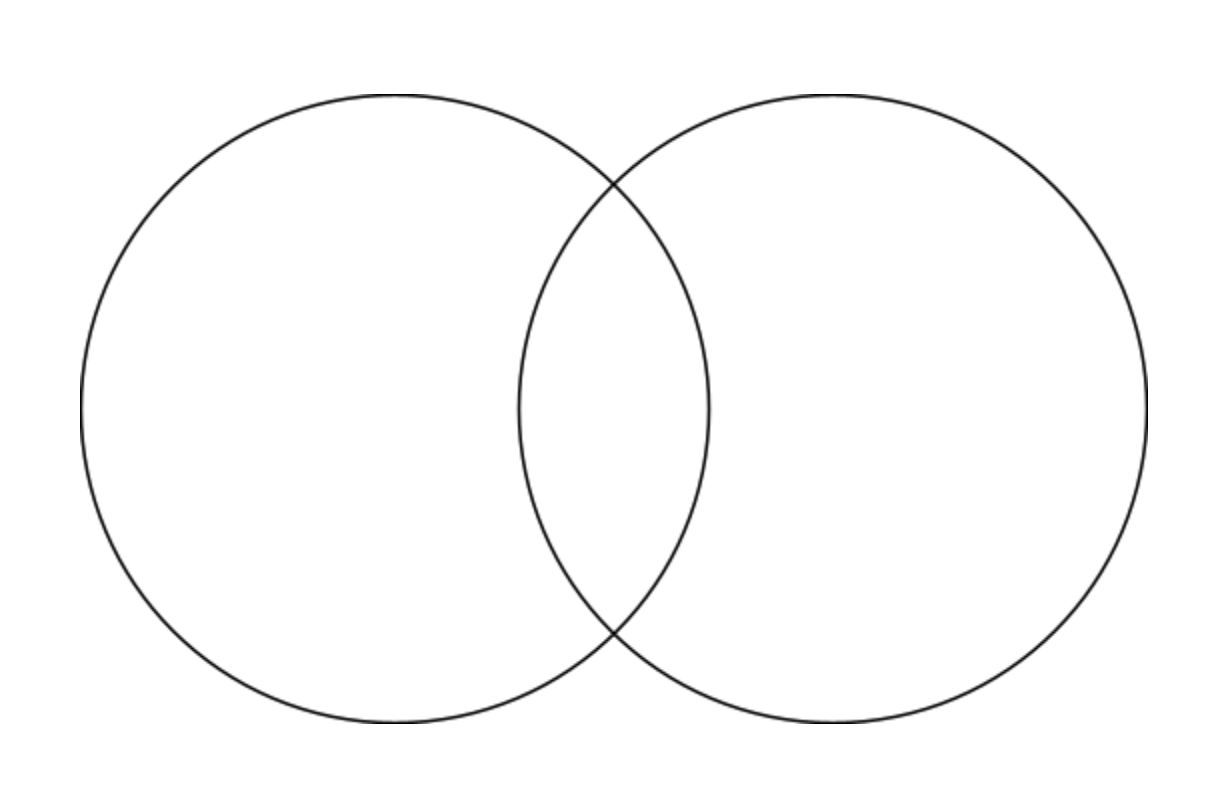
\includegraphics[width=0.6\textwidth]{venn-diagram}
    \centering
  \end{figure}

  In the above diagram, we assume the left circle corresponds to set $A$ and the
    right circle corresponds to $B$.
  The the possible sets we can make via the specified operators are:

  \begin{itemize}
    \item $A - B$, the left circle excluding the overlapping region.
    \item $A \cap B$, the overlapping region.
    \item $B - A$, the right circle excluding the overlapping region.
    \item $(A \cup B) \cap A$, the left circle.
    \item $(A \cup B) \cap B$, the right circle.
    \item $(A - B) \cup (B - A)$, the symmetric difference.
    \item $A \cup B$, the entire diagram.
  \end{itemize}

\end{proof}

\subsection{\verified{Exercise 2.19}}%
\label{sub:exercise-2.19}

Is $\powerset{(A - B)}$ always equal to $\powerset{A} - \powerset{B}$?
Is it ever equal to $\powerset{A} - \powerset{B}$?

\begin{proof}

  \lean{Bookshelf/Enderton/Set/Chapter\_2}
    {Enderton.Set.Chapter\_2.exercise\_2\_19}

  Let $A$ and $B$ be arbitrary sets.
  We show (i) that $\emptyset \in \powerset{(A - B})$ and (ii)
    $\emptyset \not\in \powerset{A} - \powerset{B}$.

  \paragraph{(i)}%
  \label{par:exercise-2.19-i}

    By definition of the \nameref{ref:power-set},
      $$\powerset{(A - B)} = \{ x \mid x \subseteq A - B \}.$$
    But $\emptyset$ is a subset of \textit{every} set.
    Thus $\emptyset \in \powerset{(A - B)}$.

  \paragraph{(ii)}%

    By the same reasoning found in \nameref{par:exercise-2.19-i},
      $\emptyset \in \powerset{A}$ and $\emptyset \in \powerset{B}$.
    But then, by definition of the relative complement,
      $\emptyset \not\in \powerset{A} - \powerset{B}$.

  \paragraph{Conclusion}%

    By the \nameref{ref:extensionality-axiom}, the two sets are never equal.

\end{proof}

\subsection{\verified{Exercise 2.20}}%
\label{sub:exercise-2.20}

Let $A$, $B$, and $C$ be sets such that $A \cup B = A \cup C$ and
  $A \cap B = A \cap C$.
Show that $B = C$.

\begin{proof}

  \lean{Bookshelf/Enderton/Set/Chapter\_2}
    {Enderton.Set.Chapter\_2.exercise\_2\_20}

  Let $A$, $B$, and $C$ be arbitrary sets.
  By the \nameref{ref:extensionality-axiom}, $B = C$ if and only if for all sets
    $x$, $x \in B \iff x \in C$.
  We prove both directions of this biconditional.

  \paragraph{($\Rightarrow$)}%

    Suppose $x \in B$.
    Then there are two cases to consider:

    \subparagraph{Case 1}%

      Assume $x \in A$.
      Then $x \in A \cap B$.
      By hypothesis, $A \cap B = A \cap C$.
      Thus $x \in A \cap C$ immediately implying $x \in C$.

    \subparagraph{Case 2}%

      Assume $x \not\in A$.
      Then $x \in A \cup B$.
      By hypothesis, $A \cup B = A \cup C$.
      Thus $x \in A \cup C$.
      Since $x \not\in A$, it follows $x \in C$.

  \paragraph{($\Leftarrow$)}%

    Suppose $x \in C$.
    Then there are two cases to consider:

    \subparagraph{Case 1}%

      Assume $x \in A$.
      Then $x \in A \cap C$.
      By hypothesis, $A \cap B = A \cap C$.
      Thus $x \in A \cap B$, immediately implying $x \in B$.

    \subparagraph{Case 2}%

      Assume $x \not\in A$.
      Then $x \in A \cup C$.
      By hypothesis, $A \cup B = A \cup C$.
      Thus $x \in A \cup B$.
      Since $x \not\in A$, it follows $x \in B$.

\end{proof}

\subsection{\verified{Exercise 2.21}}%
\label{sub:exercise-2.21}

Show that $\bigcup (A \cup B) = \bigcup A \cup \bigcup B$.

\begin{proof}

  \lean{Bookshelf/Enderton/Set/Chapter\_2}
    {Enderton.Set.Chapter\_2.exercise\_2\_21}

  Let $A$ and $B$ be arbitrary sets.
  By the \nameref{ref:extensionality-axiom}, the specified equality holds if and
    only if for all sets $x$,
    $$x \in \bigcup (A \cup B) \iff x \in \bigcup A \cup \bigcup B.$$
  We prove both directions of this biconditional.

  \paragraph{($\Rightarrow$)}%

    Suppose $x \in \bigcup (A \cup B)$.
    By definition of the union of sets, there exists some $b \in A \cup B$ such
      that $x \in b$.
    If $b \in A$, then $x \in \bigcup A$ and $x \in \bigcup A \cup \bigcup B$.
    Alternatively, if $b \in B$, then $x \in \bigcup B$ and
      $x \in \bigcup A \cup \bigcup B$.
    Regardless, $x$ is in the target set.

  \paragraph{($\Leftarrow$)}%

    Suppose $x \in \bigcup A \cup \bigcup B$.
    Then $x \in \bigcup A$ or $x \in \bigcup B$.
    WLOG, suppose $x \in \bigcup A$.
    By definition of the union of sets, there exists some $b \in A$ such that
      $x \in b$.
    But then $b \in A \cup B$ meaning $x$ is also a member of
      $\bigcup (A \cup B)$.

\end{proof}

\subsection{\verified{Exercise 2.22}}%
\label{sub:exercise-2.22}

Show that if $A$ and $B$ are nonempty sets, then
  $\bigcap (A \cup B) = \bigcap A \cap \bigcap B$.

\begin{proof}

  \lean{Bookshelf/Enderton/Set/Chapter\_2}
    {Enderton.Set.Chapter\_2.exercise\_2\_22}

  Let $A$ and $B$ be arbitrary, nonempty sets.
  By the \nameref{ref:extensionality-axiom}, the specified equality holds if and
    only if for all sets $x$,
    \begin{equation}
      \label{sub:exercise-2.22-eq1}
      x \in \bigcap (A \cup B) \iff x \in \bigcap A \cap \bigcap B.
    \end{equation}
  We prove both directions of this biconditional.

  \paragraph{($\Rightarrow$)}%

    Suppose $x \in \bigcap (A \cup B)$.
    Then for all $b \in A \cup B$, $x \in B$.
    In other words, for every member $b_1$ of $A$ and every member $b_2$ of $B$,
      $x$ is a member of both $b_1$ and $b_2$.
    But that implies $x \in \bigcap A$ and $x \in \bigcap B$.

  \paragraph{($\Leftarrow$)}%

    Suppose $x \in \bigcap A \cap \bigcap B$.
    That is, $x \in \bigcap A$ and $x \in \bigcap B$.
    By definition of the intersection of sets, forall sets $b$, if $b \in A$,
      then $x \in b$.
    Likewise, if $b \in B$, then $x \in b$.
    In other words, if $b$ is a member of either $A$ or $B$, $x \in b$.
    That immediately implies $x \in \bigcap (A \cup B$.

\end{proof}

\subsection{\unverified{Exercise 2.23}}%
\label{sub:exercise-2.23}

Show that if $\mathscr{B}$ is nonempty, then
  $A \cup \bigcap \mathscr{B} = \bigcap\; \{A \cup X \mid X \in \mathscr{B} \}$.

\begin{proof}

  Refer to \nameref{sub:general-distributive-laws}.

\end{proof}

\subsection{\verified{Exercise 2.24a}}%
\label{sub:exercise-2.24a}

Show that if $\mathscr{A}$ is nonempty, then
  $\powerset{\bigcap\mathscr{A}} =
    \bigcap\; \{\powerset{X} \mid X \in \mathscr{A} \}$.

\begin{proof}

  \lean{Bookshelf/Enderton/Set/Chapter\_2}
    {Enderton.Set.Chapter\_2.exercise\_2\_24a}

  Suppose $\mathscr{A}$ is a nonempty set.
  Then $\bigcap \mathscr{A}$ is well-defined.
  Therefore
    \begin{align*}
      \powerset{\bigcap\mathscr{A}}
        & = \{ x \mid x \subseteq \bigcap \mathscr{A} \}
          & \textref{ref:power-set} \\
        & = \{ x \mid x \subseteq
          \{ y \mid \forall X \in \mathscr{A}, y \in X \} \}
          & \text{def'n intersection} \\
        & = \{ x \mid \forall t \in x,
          t \in \{ y \mid \forall X \in \mathscr{A}, y \in X \} \}
          & \text{def'n subset} \\
        & = \{ x \mid \forall t \in x,
          (\forall X \in \mathscr{A}, t \in X) \} \\
        & = \{ x \mid \forall X \in \mathscr{A},
          (\forall t \in x, t \in X) \} \\
        & = \{ x \mid \forall X \in \mathscr{A}, x \subseteq X \} \\
        & = \{ x \mid \forall X \in \mathscr{A}, x \in \powerset{X} \}
          & \textref{ref:power-set-axiom} \\
        & = \{ x \mid
          \forall t \in \{ \powerset{X} \mid X \in \mathscr{A} \}, x \in t \} \\
        & = \bigcap\; \{\powerset{X} \mid X \in \mathscr{A}\}.
    \end{align*}

\end{proof}

\subsection{\verified{Exercise 2.24b}}%
\label{sub:exercise-2.24b}

Show that
  \begin{equation}
    \label{sub:exercise-2.24b-eq1}
    \bigcup\; \{ \powerset{X} \mid X \in \mathscr{A} \} \subseteq
      \powerset{\bigcup\mathscr{A}}.
  \end{equation}
Under what conditions does equality hold?

\begin{proof}

  \lean{Bookshelf/Enderton/Set/Chapter\_2}
    {Enderton.Set.Chapter\_2.exercise\_2\_24b}

  We first prove \eqref{sub:exercise-2.24b-eq1}.
  Let $x \in \bigcup\; \{ \powerset{X} \mid X \in \mathscr{A} \}$.
  By definition of the union of sets,
    $(\exists X \in \mathscr{A}), x \in \powerset{X}$.
  By definition of the \nameref{ref:power-set}, $x \subseteq X$.
  By \nameref{sub:exercise-2.3}, $X \subseteq \bigcup \mathscr{A}$.
  Therefore $x \subseteq \bigcup \mathscr{A}$, proving
    $x \in \powerset{\mathscr{A}}$ as expected.

  \suitdivider

  \noindent
  We show $\powerset{\bigcup A} \subseteq 
    \bigcup\;\{ \powerset{X} \mid X \in \mathscr{A} \}$ if and only if
    $\bigcup\mathscr{A} \in \mathscr{A}$.

  \paragraph{($\Rightarrow$)}%

    Suppose $\powerset{\bigcup\mathscr{A}} \subseteq
      \bigcup\;\{ \powerset{X} \mid X \in \mathscr{A} \}$.
    By definition of the \nameref{ref:power-set},
      $\bigcup\mathscr{A} \in \powerset{\bigcup\mathscr{A}}$.
    By hypothesis, $\bigcup\mathscr{A} \in 
      \bigcup\;\{ \powerset{X} \mid X \in \mathscr{A} \}$.
    By definition of the union of sets, there exists some $X \in \mathscr{A}$
      such that $\bigcup\mathscr{A} \in \powerset{X}$.
    That is, $\bigcup\mathscr{A} \subseteq X$.
    But $\bigcup\mathscr{A}$ cannot be a proper subset of $X$ since
      $X \in \mathscr{A}$.
    Thus $\bigcup\mathscr{A} = X$.
    This proves $\bigcup\mathscr{A} \in
      \bigcup\;\{ \powerset{X} \mid X \in \mathscr{A} \}$.

  \paragraph{($\Leftarrow$)}%

    Suppose $\bigcup\mathscr{A} \in A$.
    Let $x \in \powerset{\bigcup\mathscr{A}}$.
    Since $\bigcup\mathscr{A} \in \mathscr{A}$, it immediately follows that
      $x \in \{\powerset{X} \mid X \in \mathscr{A}\}$.

  \paragraph{Conclusion}%

    Equality follows immediately from this fact in conjunction with the proof
      of \eqref{sub:exercise-2.24b-eq1}.

\end{proof}

\subsection{\verified{Exercise 2.25}}%
\label{sub:exercise-2.25}

Is $A \cup \bigcup \mathscr{B}$ always the same as
  $\bigcup\;\{ A \cup X \mid X \in \mathscr{B} \}$?
If not, then under what conditions does equality hold?

\begin{proof}

  \lean{Bookshelf/Enderton/Set/Chapter\_2}
    {Enderton.Set.Chapter\_2.exercise\_2\_25}

  We prove that
    \begin{equation}
      \label{sub:exercise-2.25-eq1}
      A \cup \bigcup \mathscr{B} =
        \bigcup\;\{ A \cup X \mid X \in \mathscr{B} \}
    \end{equation}
    if and only if $A = \emptyset$ or $\mathscr{B} \neq \emptyset$.
  We prove both directions of this biconditional.

  \paragraph{($\Rightarrow$)}%

    Suppose \eqref{sub:exercise-2.25-eq1} holds true.
    There are two cases to consider:

    \subparagraph{Case 1}%

      Suppose $B \neq \emptyset$.
      Then $A = \emptyset \lor \mathscr{B} \neq \emptyset$ holds trivially.

    \subparagraph{Case 2}%

      Suppose $B = \emptyset$.
      Then $$A \cup \bigcup \mathscr{B} = A \cup \bigcup \emptyset = A$$ and
        $$
          \bigcup\;\{ A \cup X \mid X \in \mathscr{B} \}
            = \bigcup \emptyset \\
            = \emptyset.
        $$
      Then by hypothesis \eqref{sub:exercise-2.25-eq1}, $A = \emptyset$.
      Then $A = \emptyset \lor \mathscr{B} \neq \emptyset$ holds trivially.

  \paragraph{($\Leftarrow$)}%

    Suppose $A = \emptyset$ or $\mathscr{B} \neq \emptyset$.
    There are two cases to consider:

    \paragraph{Case 1}%

      Suppose $A = \emptyset$.
      Then $A \cup \bigcup \mathscr{B} = \bigcup{\mathscr{B}}$.
      Likewise,
        $$
          \bigcup \{ A \cup X \mid X \in \mathscr{B} \}
            = \bigcup \{ X \mid X \in \mathscr{B} \} \\
            = \bigcup \mathscr{B}.
        $$
      Therefore \eqref{sub:exercise-2.25-eq1} holds.

    \paragraph{Case 2}%

      Suppose $B \neq \emptyset$.
      Then
        \begin{align*}
          A \cup \bigcup\mathscr{B}
            & = \{ x \mid x \in A \lor x \in \bigcup\mathscr{B} \} \\
            & = \{ x \mid x \in A \lor (\exists b \in \mathscr{B}) x \in b \} \\
            & = \{ x \mid (\exists b \in \mathscr{B}) x \in A \lor x \in b \} \\
            & = \{ x \mid (\exists b \in \mathscr{B}) x \in A \cup b \} \\
            & = \{ x \mid x \in \bigcup \{ A \cup X \mid X \in \mathscr{B} \} \\
            & = \bigcup \{ A \cup X \mid X \in \mathscr{B} \}.
        \end{align*}
      Therefore \eqref{sub:exercise-2.25-eq1} holds.

\end{proof}

\chapter{Relations and Functions}%
\label{chap:relations-functions}

\section{Ordered Pairs}%
\label{sec:ordered-pairs}

\subsection{\verified{Theorem 3A}}%
\label{sub:theorem-3a}

\begin{theorem}[3A]

  For any sets $x$, $y$, $u$, and $v$,
    \begin{equation}
      \label{sub:theorem-3a-eq1}
      \left< u, v \right> = \left< x, y \right> \iff u = x \land v = y.
    \end{equation}

\end{theorem}

\begin{proof}

  \lean{Bookshelf/Enderton/Set/Chapter\_3}
    {Enderton.Set.Chapter\_3.OrderedPair.ext\_iff}

  Let $x$, $y$, $u$, and $v$ be arbitrary sets.

  \paragraph{($\Leftarrow$)}%

    This follows trivially.

  \paragraph{($\Rightarrow$)}%

    Suppose $\left< u, v \right> = \left< x, y \right>$.
    Then, by definition of an \nameref{ref:ordered-pair},
      \begin{equation}
        \label{sub:theorem-3a-eq2}
        \{\{u\}, \{u, v\}\} = \{\{x\}, \{x, y\}\}.
      \end{equation}
    By the \nameref{ref:extensionality-axiom}, it follows
      $\{u\} \in \{\{x\}, \{x, y\}\}$ and
      $\{u, v\} \in \{\{x\}, \{x, y\}\}$.
    That is,
      $$\{u\} = \{x\} \quad\text{or}\quad \{u\} = \{x, y\}$$
      and
      $$\{u, v\} = \{x\} \quad\text{or}\quad \{u, v\} = \{x, y\}.$$
    There are 4 cases to consider:

    \paragraph{Case 1}%

      Suppose $\{u\} = \{x\}$ and $\{u, v\} = \{x\}$.
      The former identity implies $u = x$.
      The latter identity implies $u = v = x$.
      Then \eqref{sub:theorem-3a-eq2} simplifies to
        $$\{\{u\}\} = \{\{x\}, \{x, y\}\},$$ meaning $x = y$.
      Thus $v = y$ as well.

    \paragraph{Case 2}%

      Suppose $\{u\} = \{x\}$ and $\{u, v\} = \{x, y\}$.
      The former identity implies $u = x$.
      Substituting into the latter identity yields $\{u, v\} = \{u, y\}$.
      This holds if and only if $v = y$.

    \paragraph{Case 3}%

      Suppose $\{u\} = \{x, y\}$ and $\{u, v\} = \{x\}$.
      The former identity implies $x = y = u$.
      Substituting into the latter yields $\{u, v\} = \{u\}$.
      Thus $u = v$ which in turn implies $v = y$.

    \paragraph{Case 4}%
      Suppose $\{u\} = \{x, y\}$ and $\{u, v\} = \{x, y\}$.
      The former identity implies $x = y = u$.
      Substituting into the latter yields $\{u, v\} = \{u\}$.
      This implies $v = u$ which in turn implies $v = y$.

    \paragraph{Conclusion}%

      These cases are exhaustive and each implies that $u = x$ and $v = y$.

\end{proof}

\subsection{\verified{Lemma 3B}}%
\label{sub:lemma-3b}

\begin{theorem}[3B]

  If $x \in C$ and $y \in C$, then
    $\left< x, y \right> \in \powerset{\powerset{C}}$.

\end{theorem}

\begin{proof}

  \lean{Bookshelf/Enderton/Set/Chapter\_3}
    {Enderton.Set.Chapter\_3.theorem\_3b}

  Let $C$ be an arbitrary set and $x, y \in C$.
  Then, by definition of the \nameref{ref:power-set},
    $\{x\}$ and $\{x, y\}$ are members of $\powerset{C}$.
  Likewise, $\{\{x\}, \{x, y\}\}$ is a member of $\powerset{\powerset{C}}$.
  By definition of an \nameref{ref:ordered-pair},
    $\left< x, y \right> = \{\{x\}, \{x, y\}\}$.
  This concludes our proof.

\end{proof}

\subsection{\verified{Corollary 3C}}%
\label{sub:corollary-3c}

\begin{theorem}[3C]

  For any sets $A$ and $B$, there is a set whose members are exactly the
    pairs $\left< x, y \right>$ with $x \in A$ and $y \in B$.

\end{theorem}

\begin{proof}

  \lean*{Mathlib/SetTheory/ZFC/Basic}{Set.prod}

  \note{The above Lean proof is a definition (i.e. an axiom). It does not prove
    such a set's existence from first principles.}

  Define $C = A \cup B$.
  Then for all $x \in A$ and for all $y \in B$, $x$ and $y$ are both in $C$.
  By \nameref{sub:lemma-3b}, it follows that
    $\left< x, y \right> \in \powerset{\powerset{C}}$.
  The \nameref{ref:power-set-axiom} indicates $\powerset{\powerset{C}}$ is
    indeed a set.
  Therefore the \nameref{ref:subset-axioms} are applicable.
  This implies the existence of a set $D$ such that
    $$\forall z, (z \in D \iff z \in \powerset{\powerset{C}} \land
      (\exists x, \exists y, x \in A \land y \in B \land
        z = \left< x, y \right>)).$$
  By construction $D$ is the set whose members are exactly the pairs
    $\left< x, y \right>$ with $x \in A$ and $y \in B$.

\end{proof}

\section{Relations}%
\label{sec:relations}

\subsection{\verified{Theorem 3D}}%
\label{sub:theorem-3d}

\begin{theorem}[3D]

  If $\left< x, y \right> \in A$, then $x$ and $y$ belong to $\bigcup\bigcup A$.

\end{theorem}

\begin{proof}

  \lean{Bookshelf/Enderton/Set/Chapter\_3}
    {Enderton.Set.Chapter\_3.theorem\_3d}

  Let $A$ be a set and $\left< x, y \right> \in A$.
  By definition of an \nameref{ref:ordered-pair},
    $$\left< x, y \right> = \{\{x\}, \{x, y\}\}.$$
  By \nameref{sub:exercise-2.3}, $\{\{x\}, \{x, y\}\} \subseteq \bigcup A$.
  Then $\{x, y\} \in \bigcup A$.
  Another application of \nameref{sub:exercise-2.3} implies
    $\{x, y\} \subseteq \bigcup\bigcup A$.
  Therefore $x, y \in \bigcup\bigcup A$.

\end{proof}

\section{Functions}%
\label{sec:functions}

\subsection{\verified{Theorem 3E}}%
\label{sub:theorem-3e}

\begin{theorem}[3E]

  For a set $F$, $\dom{(F^{-1})} = \ran{F}$ and $\ran{(F^{-1})} = \dom{F}$.
  For a relation $F$, $(F^{-1})^{-1} = F$.

\end{theorem}

\begin{proof}

  \statementpadding

  \lean*{Bookshelf/Enderton/Set/Relation}
    {Set.Relation.dom\_inv\_eq\_ran\_self}

  \lean*{Bookshelf/Enderton/Set/Relation}
    {Set.Relation.ran\_inv\_eq\_dom\_self}

  \lean{Bookshelf/Enderton/Set/Relation}
    {Set.Relation.inv\_inv\_eq\_self}

  We prove that (i) $\dom{(F^{-1})} = \ran{F}$, (ii) $\ran{(F^{-1})} = \dom{F}$,
    and (iii) $(F^{-1})^{-1} = F$.

  \paragraph{(i)}%

    By definition of the \nameref{ref:domain}, $x \in \dom{(F^{-1})}$ if and
      only if there exists some $y$ such that $\left< x, y \right> \in F^{-1}$.
    By definition of the \nameref{ref:inverse} of a set,
      $\left< y, x \right> \in F$.
    By definition of the \nameref{ref:range}, $x \in \ran{F}$.
    Since each step holds biconditionally, it follows
      $\dom{(F^{-1})} = \ran{F}$ as expected.

  \paragraph{(ii)}%

    By definition of the \nameref{ref:range}, $x \in \ran{(F^{-1})}$ if and
      only if there exists some $t$ such that $\left< t, x \right> \in F^{-1}$.
    By definition of the \nameref{ref:inverse} of a set,
      $\left< x, t \right> \in F$.
    By definition of the \nameref{ref:domain}, $x \in \dom{F}$.
    Since each step holds biconditionally, it follows
      $\ran{(F^{-1})} = \dom{F}$.

  \paragraph{(iii)}%

    By definition of the \nameref{ref:inverse} of a set,
      \begin{align*}
        (F^{-1})^{-1}
          & = \{\left< u, v \right> \mid \left< v, u \right> \in F^{-1}\} \\
          & = \{\left< u, v \right> \mid \left< u, v \right> \in F\} \\
          & = F.
      \end{align*}

\end{proof}

\subsection{\verified{Theorem 3F}}%
\label{sub:theorem-3f}

\begin{theorem}[3F]

  For a set $F$, $F^{-1}$ is a function iff $F$ is single-rooted.
  A relation $F$ is a function iff $F^{-1}$ is single-rooted.

\end{theorem}

\begin{proof}

  \statementpadding

  \lean*{Bookshelf/Enderton/Set/Relation}
    {Set.Relation.single\_valued\_inv\_iff\_single\_rooted\_self}

  \lean{Bookshelf/Enderton/Set/Relation}
    {Set.Relation.single\_valued\_self\_iff\_single\_rooted\_inv}

  We prove that (i) any set $F$, $F^{-1}$ is a function iff $F$ is
    single-rooted and (ii) any relation $F$ is a function iff $F^{-1}$ is
    single-rooted.

  \paragraph{(i)}%
  \label{par:theorem-3f-i}

    Let $F$ be any set.

    \subparagraph{($\Rightarrow$)}%

      Suppose $F^{-1}$ is a \nameref{ref:function}.
      By definition, for each $x \in \dom{(F^{-1})}$, there is only one $y$
        such that $\left< x, y \right> \in F^{-1}$.
      By definition of the \nameref{ref:inverse} of $F$,
        $F^{-1} = \{\left< u, v \right> \mid vFu\}$.
      Then for each $x \in \ran{F}$, there exists exactly one $y$ such that
        $\left< y, x \right> \in F$.
      This definitionally means $F$ is single-rooted.

    \subparagraph{($\Leftarrow$)}%

      Suppose $F$ is single-rooted.
      By definition, for each $x \in \ran{F}$, there is only one $t$ such that
        $\left< t, x \right> \in F$.
      By definition of the \nameref{ref:inverse} of $F$,
        $F^{-1} = \{\left< u, v \right> \mid vFu\}$.
      Then for each $x \in \dom{(F^{-1})}$ there exists exactly one $t$ such
        that $\left< x, t \right> \in F^{-1}$.
      This definitionally means $F^{-1}$ is a function.

  \paragraph{(ii)}%

    Let $F$ be a \nameref{ref:relation}.

    \subparagraph{($\Rightarrow$)}%

      Suppose $F$ is a function.
      By \nameref{sub:theorem-3e}, $F = (F^{-1})^{-1}$.
      Then by \nameref{par:theorem-3f-i}, $F^{-1}$ is single-rooted.

    \subparagraph{($\Leftarrow$)}%

      Suppose $F^{-1}$ is single-rooted.
      Then by \nameref{par:theorem-3f-i}, $(F^{-1})^{-1}$ is a function.
      By \nameref{sub:theorem-3e}, $(F^{-1})^{-1} = F$.
      Thus $F$ is a function.

\end{proof}

\subsection{\verified{Lemma 1}}%
\label{sub:lemma-1}

For any one-to-one function $F$, $F^{-1}$ is also one-to-one.

\begin{proof}

  \lean{Bookshelf/Enderton/Set/Relation}
    {Set.Relation.one\_to\_one\_self\_iff\_one\_to\_one\_inv}

  We prove that (i) $F^{-1}$ is a function and (ii) $F^{-1}$ is single-rooted.

  \paragraph{(i)}%
  \label{par:lemma-1-i}

    By hypothesis, $F$ is one-to-one.
    This means it is single-rooted, i.e. for all $x \in \ran{F}$, there exists
      exactly one $t$ such that $\left< t, x \right> \in F$.
    By definition of the \nameref{ref:inverse} of $F$,
      $\left< x, t \right> \in F^{-1}$.
    But then for all $x \in \dom{(F^{-1})}$, there exists exactly one $t$ such
      that $\left< x, t \right> \in F^{-1}$.
    Thus $F^{-1}$ is a function.

  \paragraph{(ii)}%
  \label{par:lemma-1-ii}

    By hypothesis, $F$ is single-valued.
    That is, for all $x \in \dom{F}$, there exists exactly one $y$ such that
      $\left< x, y \right> \in F$.
    By definition of the \nameref{ref:inverse} of $F$,
      $\left< y, x \right> \in F^{-1}$.
    But then for all $x \in \ran{(F^{-1})}$, there exists exactly one $y$ such
      that $\left< y, x \right> \in F^{-1}$.
    Thus $F^{-1}$ is single-rooted.

  \paragraph{Conclusion}%

    By \nameref{par:lemma-1-i} and \nameref{par:lemma-1-ii}, $F^{-1}$ is
      a one-to-one function.

\end{proof}

\subsection{\verified{Theorem 3G}}%
\label{sub:theorem-3g}

\begin{theorem}[3G]

  Assume that $F$ is a one-to-one function.
  If $x \in \dom{F}$, then $F^{-1}(F(x)) = x$.
  If $y \in \ran{F}$, then $F(F^{-1}(y)) = y$.

\end{theorem}

\begin{proof}

  \statementpadding

  \lean*{Bookshelf/Enderton/Set/Chapter\_3}
    {Enderton.Set.Chapter\_3.theorem\_3g\_i}

  \lean{Bookshelf/Enderton/Set/Chapter\_3}
    {Enderton.Set.Chapter\_3.theorem\_3g\_ii}

  Suppose $F$ is a one-to-one \nameref{ref:function}.
  Then \nameref{sub:lemma-1} indicates $F^{-1}$ is a one-to-one function with
    domain $\ran{F}$ and range $\dom{F}$.

  For all $x \in \dom{F}$, $\left< x, F(x) \right> \in F$.
  Then $\left< F(x), x \right> \in F^{-1}$.
  Since $F^{-1}$ is single-valued, $F^{-1}(F(x)) = x$.

  For all $y \in \ran{F}$, $\left< y, F^{-1}(y) \right> \in F^{-1}$.
  Then $\left< F^{-1}(y), y \right> \in F$.
  Since $F$ is single-valued, $F(F^{-1}(y)) = y$.

\end{proof}

\subsection{\verified{Theorem 3H}}%
\label{sub:theorem-3h}

\begin{theorem}[3H]

  Assume that $F$ and $G$ are functions.
  Then $F \circ G$ is a function, its domain is
    \begin{equation}
      \label{sub:theorem-3h-eq1}
      \{x \in \dom{G} \mid G(x) \in \dom{F}\},
    \end{equation}
    and for $x$ in its domain, $(F \circ G)(x) = F(G(x))$.

\end{theorem}

\begin{proof}

  \statementpadding

  \lean*{Bookshelf/Enderton/Set/Relation}
    {Set.Relation.single\_valued\_comp\_is\_single\_valued}

  \lean{Bookshelf/Enderton/Set/Chapter\_3}
    {Enderton.Set.Chapter\_3.theorem\_3h\_dom}

  Let $F$ and $G$ be \nameref{ref:function}s.
  By definition of the \nameref{ref:composition} of $F$ and $G$,
    \begin{equation}
      \label{sub:theorem-3h-eq2}
      F \circ G = \{\left< u, v \right> \mid \exists t(uGt \land tFv)\}.
    \end{equation}
  By construction, $F \circ G$ is a relation.
  By the definition of the \nameref{ref:domain} of a relation,
    $x \in \dom{(F \circ G)}$ if and only if there exists some $y$ such that
    $\left< x, y \right> \in F \circ G$.
  We prove that (i) $F \circ G$ is a function with domain satisfying
    \eqref{sub:theorem-3h-eq1}, and (ii) $(F \circ G)(x) = F(G(x))$.

  \paragraph{(i)}%
  \label{par:theorem-3h-i}

    By \eqref{sub:theorem-3h-eq2}, there exists some $t$ such that
      $\left< x, t \right> \in G$ and $\left< t, y \right> \in F$.
    Since $G$ is single-valued, $t$ is uniquely determined by $x$.
    Since $F$ is single-valued, $y$ is uniquely determined by $t$.
    Therefore, by transitivity, $y$ is uniquely determined by $x$.
    Thus $F \circ G$ is single-valued, i.e. $F \circ G$ is a function.

    Furthermore, by definition of function application, $t = G(x)$.
    Thus
      $$\left< x, G(x) \right> \in G \quad\text{and}\quad
        \left< G(x), y \right> \in F.$$
    This immediately implies \eqref{sub:theorem-3h-eq1} holds true.

  \paragraph{(ii)}%

    Let $x \in \dom{(F \circ G)}$.
    By definition, $\left< x, (F \circ G)(x) \right> \in F \circ G$.
    Then \eqref{sub:theorem-3h-eq2} implies $(F \circ G)(x)$ satisfies
      $\left< G(x), (F \circ G)(x) \right> \in F$.
    This is equivalent to saying $F(G(x)) = (F \circ G)(x)$ as expected.

\end{proof}

\subsection{\verified{Theorem 3I}}%
\label{sub:theorem-3i}

\begin{theorem}[3I]

  For any sets $F$ and $G$, $$(F \circ G)^{-1} = G^{-1} \circ F^{-1}.$$

\end{theorem}

\begin{proof}

  \lean{Bookshelf/Enderton/Set/Relation}
    {Set.Relation.comp\_inv\_eq\_inv\_comp\_inv}

  By definition of the \nameref{ref:composition} of $F$ and $G$,
    $$F \circ G = \{\left< u, v \right> \mid \exists t(uGt \land tFv)\}.$$
  By definition of the \nameref{ref:inverse} of a function,
    \begin{align*}
      (F \circ G)^{-1}
        & = \{\left< u, v \right> \mid \exists t (vGt \land tFu)\} \\
        & = \{\left< u, v \right> \mid \exists t (tFu \land vGt)\} \\
        & = \{\left< u, v \right> \mid
          \exists t \left[ u(F^{-1})t \land t(G^{-1})v \right]\} \\
        & = G^{-1} \circ F^{-1}.
    \end{align*}

\end{proof}

\subsection{\pending{Theorem 3J}}%
\label{sub:theorem-3j}

\begin{theorem}[3J]

  Assume that $F \colon A \rightarrow B$, and that $A$ is nonempty.
  \begin{enumerate}[(a)]
    \item There exists a function $G \colon B \rightarrow A$ (a "left inverse")
      such that $G \circ F$ is the identity function $I_A$ on $A$ iff $F$ is
      one-to-one.
    \item There exists a function $H \colon B \rightarrow A$ (a "right inverse")
      such that $F \circ H$ is the identity function $I_B$ on $B$ iff $F$ maps
      $A$ \textit{onto} $B$.
  \end{enumerate}

\end{theorem}

\begin{proof}

  Let $F$ be a \nameref{ref:function} from nonempty set $A$ to set $B$.

  \paragraph{(a)}%

    We prove there exists a function $G \colon B \rightarrow A$ such that
      $G \circ F = I_A$ if and only if $F$ is one-to-one.

    \subparagraph{($\Rightarrow$)}%

      Let $G \colon B \rightarrow A$ such that $G \circ F = I_A$.
      All that remains is to prove $F$ is single-rooted.
      Let $y \in \ran{F}$.
      By definition of the \nameref{ref:range} of a function, there exists some
        $x_1$ such that $\left< x_1, y \right> \in F$.
      Suppose there exists a set $x_2$ such that $\left< x_2, y \right> \in F$.
      By hypothesis, $G(F(x_1)) = G(F(x_2))$ implies $I_A(x_1) = I_A(x_2)$.
      Thus $x_1 = x_2$.
      Therefore $F$ must be single-rooted.

    \subparagraph{($\Leftarrow$)}%

      Let $F$ be one-to-one.
      Since $A$ is nonempty, there exists some $a \in A$.
      Let $G \colon B \rightarrow A$ be given by
        $$G(y) = \begin{cases}
          F^{-1}(y) & \text{if } y \in \ran{F} \\
          a & \text{otherwise}.
        \end{cases}$$
      $G$ is a function by virtue of \nameref{sub:lemma-1} and choice of mapping
        for all values $y \not\in \ran{F}$.
      Furthermore, for all $x \in A$, $F(x) \in \ran{F}$.
      Thus $(G \circ F)(x) = G(F(x)) = F^{-1}(F(x)) = x$ by
        \nameref{sub:theorem-3g}.

  \paragraph{(b)}%

    We prove there exists a function $H \colon B \rightarrow A$ such that
      $F \circ H = I_A$ if and only if $F$ maps $A$ onto $B$.

    \subparagraph{($\Rightarrow$)}%

      Suppose $H \colon B \rightarrow A$ such that $F \circ H = I_A$.
      All that remains is to prove $\ran{F} = B$.
      Note that $\ran{F} \subseteq B$ by hypothesis.
      Let $y \in B$.
      But $F(H(y)) = y$ meaning $y \in \ran{F}$.
      Thus $B \subseteq \ran{F}$.
      Since $\ran{F} \subseteq B$ and $B \subseteq \ran{F}$, $\ran{F} = B$.

    \subparagraph{($\Leftarrow$)}%

      Suppose $F$ maps $A$ \textit{onto} $B$.
      By definition of maps onto, $\ran{F} = B$.
      Then for all $y \in B$, there exists some $x \in A$ such that
        $\left< x, y \right> \in F$.
      Notice though that $F^{-1}[\{y\}]$ may not be a singleton set.
      Then there is no obvious way to \textit{choose} an element from each
        preimage to form a function.
      By the \nameref{ref:axiom-of-choice-1}, there exists a function
        $H \subseteq F^{-1}$ such that $\dom{H} = \dom{F^{-1}} = B$.
      For all $y \in B$, $\left< y, H(y) \right> \in H \subseteq F^{-1}$
        meaning $\left< H(y), y \right> \in F$.
      Thus $F(H(y)) = y$ as expected.

\end{proof}

\subsection{\verified{Theorem 3K(a)}}%
\label{sub:theorem-3k-a}

\begin{theorem}[3K(a)]

  The following hold for any sets. ($F$ need not be a function.)
  The image of a union is the union of the images:
    \begin{equation}
      \label{sub:theorem-3k-a-eq1}
      \img{F}{A \cup B} = \img{F}{A} \cup \img{F}{B}
    \end{equation}
    and
    \begin{equation}
      \label{sub:theorem-3k-a-eq2}
      \img{F}{\bigcup{\mathscr{A}}} =
        \bigcup\;\{\img{F}{A} \mid A \in \mathscr{A}\}.
    \end{equation}

\end{theorem}

\begin{proof}

  \lean{Bookshelf/Enderton/Set/Chapter\_3}
    {Enderton.Set.Chapter\_3.theorem\_3k\_a}

  Let $F$, $A$, $B$, and $\mathscr{A}$ be arbitrary sets.
  We prove (i) \eqref{sub:theorem-3k-a-eq1} and (ii)
    \eqref{sub:theorem-3k-a-eq2}.

  \paragraph{(i)}%

    By definition of the \nameref{ref:image} of a set:
      \begin{align*}
        \img{F}{A \cup B}
          & = \{v \mid \exists u, u \in A \cup B \land uFv\} \\
          & = \{v \mid \exists u,
            (u \in A \land uFv) \lor (u \in B \land uFv)\} \\
          & = \{v \mid (\exists u \in A) uFv\} \cup
            \{v \mid (\exists u \in B) uFv\} \\
          & = \img{F}{A} \cup \img{F}{B}.
      \end{align*}

  \paragraph{(ii)}%

    We prove that both sides of \eqref{sub:theorem-3k-a-eq2} is a subset of the
      other.

    \subparagraph{($\subseteq$)}%

      Let $v \in \img{F}{\bigcup{\mathscr{A}}}$.
      By definition of the \nameref{ref:image} of a set, there exists a set $u$
        such that $u \in \bigcup{\mathscr{A}} \land uFv$.
      Then, by definition of the union of sets, there exists some
        $A \in \mathscr{A}$ such that $u \in A$.
      Therefore $v \in \img{F}{A}$ meaning
        $v \in \bigcup\{\img{F}{A} \mid A \in \mathscr{A}\}$.

    \subparagraph{($\supseteq$)}%

      Let $v \in \bigcup\{\img{F}{A} \mid A \in \mathscr{A}\}$.
      Then there exists some $b \in \{\img{F}{A} \mid A \in \mathscr{A}\}$ such
        that $v \in b$.
      In other words, there exists some $A \in \mathscr{A}$ such that
        $v \in b = \img{F}{A}$.
      By definition of the \nameref{ref:image} of a set, there exists a set $u$
        such that $u \in A \land uFv$.
      But this implies that $u \in \bigcup{\mathscr{A}} \land uFv$.
      Therefore $v \in \img{F}{\bigcup{\mathscr{A}}}$.

\end{proof}

\subsection{\verified{Theorem 3K(b)}}%
\label{sub:theorem-3k-b}

\begin{theorem}[3K(b)]

  The following hold for any sets. ($F$ need not be a function.)
  The image of an intersection is included in the intersection of the images:
    \begin{equation}
      \label{sub:theorem-3k-b-eq1}
      \img{F}{A \cap B} \subseteq \img{F}{A} \cap \img{F}{B}
    \end{equation}
    and
    \begin{equation}
      \label{sub:theorem-3k-b-eq2}
      \img{F}{\bigcap\mathscr{A}} \subseteq
        \bigcap\;\{\img{F}{A} \mid A \in \mathscr{A}\}.
    \end{equation}
    for nonempty $\mathscr{A}$.
  Equality holds if $F$ is single-rooted.

\end{theorem}

\begin{proof}

  \statementpadding

  \lean*{Bookshelf/Enderton/Set/Chapter\_3}
    {Enderton.Set.Chapter\_3.theorem\_3k\_b\_i}

  \lean{Bookshelf/Enderton/Set/Chapter\_3}
    {Enderton.Set.Chapter\_3.theorem\_3k\_b\_ii}

  Let $F$, $A$, $B$ be arbitrary sets.
  Let $\mathscr{A}$ be a nonempty set.
  We first prove (i) \eqref{sub:theorem-3k-b-eq1} and (ii)
    \eqref{sub:theorem-3k-b-eq2}.
  Then, assuming $F$ is single-rooted, we prove both (iii)
    \eqref{sub:theorem-3k-b-eq1} and (iv) \eqref{sub:theorem-3k-b-eq2} hold
    under equality.

  \paragraph{(i)}%
  \label{par:theorem-3k-b-i}

    Let $v \in \img{F}{A \cap B}$.
    By definition of the \nameref{ref:image} of a set,
      $\exists u \in A \cap B, uFv$.
    Then $u \in A \land uFv$ and $u \in B \land uFv$.
    Therefore $v \in \img{F}{A} \cap \img{F}{B}$.

  \paragraph{(ii)}%
  \label{par:theorem-3k-b-ii}

    Let $v \in \img{F}{\bigcap{\mathscr{A}}}$.
    By definition of the \nameref{ref:image} of a set,
      $\exists u \in \bigcap{\mathscr{A}}, uFv$.
    Then $\exists u, (\forall A \in \mathscr{A}, u \in A) \land uFv$.
    This implies that $\forall A \in \mathscr{A}, \exists u \in A, uFv$.
    Then $\forall A \in \mathscr{A}, v \in \img{F}{A}$.
    Thus $v \in \bigcap\{\img{F}{A} \mid A \in \mathscr{A}\}$.

  \paragraph{(iii)}%

    Suppose $F$ is single-rooted.
    By \nameref{par:theorem-3k-b-i},
      $$\img{F}{A \cap B} \subseteq \img{F}{A} \cap \img{F}{B}.$$
    All that remains is showing
      $$\img{F}{A} \cap \img{F}{B} \subseteq \img{F}{A \cap B}.$$
    Let $v \in \img{F}{A} \cap \img{F}{B}$.
    Then $v \in \img{F}{A}$ and $v \in \img{F}{B}$.
    That is, $\exists u \in A, uFv$ and $\exists w \in B, wFv$.
    Since $F$ is single rooted, it follows $u = w$.
    Thus $u \in A \cap B \land uFv$ meaning $v \in \img{F}{A \cap B}$.

  \paragraph{(iv)}%

    Suppose $F$ is single-rooted.
    By \nameref{par:theorem-3k-b-ii},
      $$\img{F}{\bigcap\mathscr{A}} \subseteq
        \bigcap\;\{\img{F}{A} \mid A \in \mathscr{A}\}.$$
    All that remains is showing
      $$\bigcap\;\{\img{F}{A} \mid A \in \mathscr{A}\} \subseteq
        \img{F}{\bigcap\mathscr{A}}.$$
    Let $v \in \bigcap\;\{\img{F}{A} \mid A \in \mathscr{A}\}$.
    Then $\forall A \in \mathscr{A}, v \in \img{F}{A}$.
    By definition of the \nameref{ref:image} of a set,
      $\forall A \in \mathscr{A}, \exists u \in A, uFv$.
    Since $F$ is single-rooted and $\mathscr{A}$ is nonempty, it follows that
      $\exists u, (\forall A \in \mathscr{A}, u \in A) \land uFv$.
    Equivalently, $\exists u \in \bigcap{A}, uFv$.
    Thus $v \in \img{F}{\bigcap{A}}$.

\end{proof}

\subsection{\verified{Theorem 3K(c)}}%
\label{sub:theorem-3k-c}

\begin{theorem}[3K(c)]

  The following hold for any sets. ($F$ need not be a function.)
  The image of a difference includes the difference of the images:
    \begin{equation}
      \label{sub:theorem-3k-c-eq1}
      \img{F}{A} - \img{F}{B} \subseteq \img{F}{A - B}.
    \end{equation}
  Equality holds if $F$ is single-rooted.

\end{theorem}

\begin{proof}

  \statementpadding

  \lean*{Bookshelf/Enderton/Set/Chapter\_3}
    {Enderton.Set.Chapter\_3.theorem\_3k\_c\_i}

  \lean{Bookshelf/Enderton/Set/Chapter\_3}
    {Enderton.Set.Chapter\_3.theorem\_3k\_c\_ii}

  We prove that (i) \eqref{sub:theorem-3k-c-eq1} holds and (ii) equality holds
    if $F$ is single-rooted.

  \paragraph{(i)}%
  \label{par:theorem-3k-c-i}

    Let $v \in \img{F}{A} - \img{F}{B}$.
    By definition of the difference of two sets,
      $v \in \img{F}{A}$ and $v \not\in \img{F}{B}$.
    By definition of the \nameref{ref:image} of a set, there exists a set
      $u \in A$ such that $\left< u, v \right> \in F$.
    Likewise, $\forall w \in B, \left< w, v \right> \not\in F$.
    Thus $u \not\in B$, since otherwise we get an immediate contradiction.
    Therefore $u \in A - B$ meaning $v \in \img{F}{A - B}$.

  \paragraph{(ii)}%

    Suppose $F$ is single-rooted.
    By \nameref{par:theorem-3k-c-i},
      $$\img{F}{A} - \img{F}{B} \subseteq \img{F}{A - B}.$$
    All that remains is showing
      $$\img{F}{A - B} \subseteq \img{F}{A} - \img{F}{B}.$$
    Let $v \in \img{F}{A - B}$.
    By definition of the \nameref{ref:image} of a set, there exists a set
      $u \in A - B$ such that $uFv$.
    Then $u \in A$ and $u \not\in B$.
    The former membership relation implies $v \in \img{F}{A}$.
    The latter implies $v \not\in \img{F}{B}$ since $F$ being single-rooted
      would otherwise invoke an immediate contradiction.
    Thus $v \in \img{F}{A} - \img{F}{B}$.

\end{proof}

\subsection{\verified{Corollary 3L}}%
\label{sub:corollary-3l}

\begin{theorem}[3L]

  For any function $G$ and sets $A$, $B$, and $\mathscr{A}$:
  \begin{align}
    \img{G^{-1}}{\bigcup{\mathscr{A}}}
      & = \bigcup\;\{\img{G^{-1}}{A} \mid A \in \mathscr{A}\},
      \label{sub:corollary-3l-eq1} \\
    \img{G^{-1}}{\bigcap{\mathscr{A}}}
      & = \bigcap\;\{\img{G^{-1}}{A} \mid A \in \mathscr{A}\}
      \text{ for } \mathscr{A} \neq \emptyset,
      \label{sub:corollary-3l-eq2} \\
    \img{G^{-1}}{A - B} & = \img{G^{-1}}{A} - \img{G^{-1}}{B}.
      \label{sub:corollary-3l-eq3}
  \end{align}

\end{theorem}

\begin{proof}

  \statementpadding

  \lean*{Bookshelf/Enderton/Set/Chapter\_3}
    {Enderton.Set.Chapter\_3.corollary\_3l\_i}

  \lean*{Bookshelf/Enderton/Set/Chapter\_3}
    {Enderton.Set.Chapter\_3.corollary\_3l\_ii}

  \lean{Bookshelf/Enderton/Set/Chapter\_3}
    {Enderton.Set.Chapter\_3.corollary\_3l\_iii}

  \nameref{sub:theorem-3k-a} implies \eqref{sub:corollary-3l-eq1}.
  Because the inverse of a function is always single-rooted,
    \nameref{sub:theorem-3k-b} implies \eqref{sub:corollary-3l-eq2}.
  Likewise \nameref{sub:theorem-3k-c} implies \eqref{sub:corollary-3l-eq3}.

\end{proof}

\section{Equivalence Relations}%
\label{sec:equivalence-relations}

\subsection{\pending{Theorem 3M}}%
\label{sub:theorem-3m}

\begin{theorem}[3M]

  If $R$ is a symmetric and transitive relation, then $R$ is an equivalence
    relation on $\fld{R}$.

\end{theorem}

\begin{proof}

  Suppose $R$ is a \nameref{ref:symmetric} and \nameref{ref:transitive}
    \nameref{ref:relation}.
  By definition, the \nameref{ref:field} of $R$ is given by
    $\fld{R} = \dom{R} \cup \ran{R}$.
  An \nameref{ref:equivalence-relation} on $\fld{R}$ is, by definition, a
    binary relation \nameref{ref:reflexive} on $\fld{R}$, symmetric, and
    transitive.
  All that remains is to show $R$ is reflexive on $\fld{R}$.

  Let $x \in \fld{R}$.
  Then $x \in \dom{R}$ or $x \in \ran{R}$.
  If $x \in \dom{R}$, there exists some $y$ such that $xRy$.
  Since $R$ is symmetric, it follows $yRx$.
  Since $R$ is transitive, it follows $xRx$.
  If instead $x \in \ran{R}$, there exists some $t$ such that $tRx$.
  Since $R$ is symmetric, it follows $xRt$.
  Since $R$ is transitive, it follows $xRx$.
  Thus $R$ is reflexive on $\fld{R}$.

\end{proof}

\subsection{\pending{Lemma 3N}}%
\label{sub:lemma-3n}

\begin{lemma}[3N]

  Assume that $R$ is an equivalence relation on $A$ and that $x$ and $y$ belong
    to $A$.
  Then $$[x]_R = [y]_R \iff xRy.$$

\end{lemma}

\begin{proof}

  Suppose $R$ is an \nameref{ref:equivalence-relation} on set $A$.
  Let $x, y \in A$.

  \paragraph{($\Rightarrow$)}%

    Suppose $[x]_R = [y]_R$.
    Since $R$ is an equivalence relation, it is reflexive on $A$.
    Thus $yRy$ meaning $y \in [y]_R = \{t \mid yRt\}$.
    Since $[x]_R = [y]_R$, $y \in \{t \mid xRt\}$ as well.
    That is, $xRy$.

  \paragraph{($\Leftarrow$)}%

    Suppose $xRy$.
    We show $[x]_R \subseteq [y]_R$ and $[y]_R \subseteq [x]_R$.

    \subparagraph{($\subseteq$)}%

      Let $t \in [x]_R$.
      Then $xRt$.
      Since $R$ is symmetric, $xRy$ implies $yRx$.
      Since $R$ is transitive, $yRx$ and $xRt$ implies $yRt$.
      Thus $t \in [y]_R$.

    \subparagraph{($\supseteq$)}%

      Let $t \in [y]_R$.
      Then $yRt$.
      Since $R$ is transitive, $xRy$ and $yRt$ implies $xRt$.
      Thus $t \in [x]_R$.

\end{proof}

\subsection{\pending{Theorem 3P}}%
\label{sub:theorem-3p}

\begin{theorem}[3P]

  Assume that $R$ is an equivalence relation on $A$.
  Then the set $\{[x]_R \mid x \in A\}$ of all equivalence classes is a
    partition of $A$.

\end{theorem}

\begin{proof}

  Let $\Pi = \{[x]_R \mid x \in A\}$.
  We show that (i) no two different sets in $\Pi$ have any common elements and
    (ii) that each element of $A$ is in some set in $\Pi$.

  \paragraph{(i)}%

    Let $[x]_R, [y]_R \in \Pi$ be two different sets.
    We must show that $[x]_R \cap [y]_R = \emptyset$.
    For the sake of contradiction, suppose $[x]_R \cap [y]_R \neq \emptyset$.
    Let $z \in [x]_R \cap [y]_R$.
    Then $xRz$ and $yRz$.
    Since $R$ is an \nameref{ref:equivalence-relation} on $A$, it is
      \nameref{ref:symmetric} and \nameref{ref:transitive}.
    Then $zRy$ and $xRy$.
    By \nameref{sub:lemma-3n}, $xRy$ if and only if $[x]_R = [y]_R$,
      contradicting the distinctness of $[x]_R$ and $[y]_R$.
    Thus it follows $[x]_R \cap [y]_R] = \emptyset$.

  \paragraph{(ii)}%

    Let $x \in A$.
    Since $R$ is an \nameref{ref:equivalence-relation} on $A$, it follows
      $xRx$.
    Thus $x$ is a member of some set in $\Pi$, namely $[x]_R$.

\end{proof}

\subsection{\sorry{Theorem 3Q}}%
\label{sub:theorem-3q}

\begin{theorem}[3Q]

  Assume that $R$ is an equivalence relation on $A$ and that
    $F \colon A \rightarrow A$.
  If $F$ is compatible with $R$, then there exists a unique
    $\hat{F} \colon A / R \rightarrow A / R$ such that
    $$\hat{F}([x]_R) = [F(x)]_R \quad\text{for all } x \text{ in } A.$$
  If $F$ is not compatible with $R$, then no such $\hat{F}$ exists.
  Analogous results apply to functions from $A \times A$ into $A$.

\end{theorem}

\begin{proof}

  TODO

\end{proof}

\section{Exercises 3}%
\label{sec:exercises-3}

\subsection{\verified{Exercise 3.1}}%
\label{sub:exercise-3.1}

Suppose that we attempted to generalize the Kuratowski definitions of ordered
  pairs to ordered triples by defining
  $$\left< x, y, z \right>^* = \{\{x\}, \{x, y\}, \{x, y, z\}\}.$$
Show that this definition is unsuccessful by giving examples of objects
  $u$, $v$, $w$, $x$, $y$, $z$ with
  $\left< x, y, z \right>^* = \left< u, v, w \right>^*$ but with either
  $y \neq v$ or $z \neq w$ (or both).

\begin{proof}

  \lean{Bookshelf/Enderton/Set/Chapter\_3}
    {Enderton.Set.Chapter\_3.exercise\_3\_1}

  Let $x = 1$, $y = 1$, and $z = 2$.
  Let $u = 1$, $v = 2$, and $w = 2$.
  Then
    \begin{align*}
      \left< x, y, z \right>^*
        & = \{\{x\}, \{x, y\}, \{x, y, z\}\} \\
        & = \{\{1\}, \{1, 1\}, \{1, 1, 2\}\} \\
        & = \{\{1\}, \{1, 2\}\}.
    \end{align*}
  Likewise
    \begin{align*}
      \left< u, v, w \right>^*
        & = \{\{u\}, \{u, v\}, \{u, v, w\}\} \\
        & = \{\{1\}, \{1, 2\}, \{1, 2, 2\}\} \\
        & = \{\{1\}, \{1, 2\}\}.
    \end{align*}
  Thus $\left< x, y, z \right>^* = \left< u, v, w \right>^*$ but $y \neq v$.

\end{proof}

\subsection{\verified{Exercise 3.2a}}%
\label{sub:exercise-3.2a}

Show that $A \times (B \cup C) = (A \times B) \cup (A \times C)$.

\begin{proof}

  \lean{Bookshelf/Enderton/Set/Chapter\_3}
    {Enderton.Set.Chapter\_3.exercise\_3\_2a}

  Let $A$, $B$, and $C$ be arbitrary sets.
  Then by \nameref{sub:corollary-3c} and the definition of the union of sets,
    \begin{align*}
      A \times (B \cup C)
        & = \{ \left< x, y \right> \mid x \in A \land y \in (B \cup C) \} \\
        & = \{ \left< x, y \right> \mid
          x \in A \land (y \in B \lor y \in C) \} \\
        & = \{ \left< x, y \right> \mid
          (x \in A \land y \in B) \lor (x \in A \land y \in C) \} \\
        & = \{ \left< x, y \right> \mid (x \in A \land y \in B) \} \cup
          \{ \left< x, y \right> \mid (x \in A \land y \in C) \} \\
        & = (A \times B) \cup (A \times C).
    \end{align*}

\end{proof}

\subsection{\verified{Exercise 3.2b}}%
\label{sub:exercise-3.2b}

Show that if $A \times B = A \times C$ and $A \neq \emptyset$, then $B = C$.

\begin{proof}

  \lean{Bookshelf/Enderton/Set/Chapter\_3}
    {Enderton.Set.Chapter\_3.exercise\_3\_2b}

  Let $A$, $B$, and $C$ be arbitrary sets such that $A \neq \emptyset$.
  By \nameref{sub:corollary-3c},
    \begin{align}
      A \times B & = \{ \left< x, y \right> \mid x \in A \land y \in B \}
        & \label{sub:exercise-3.2b-eq1} \\
      A \times C & = \{ \left< x, y \right> \mid x \in A \land y \in C \}.
        & \label{sub:exercise-3.2b-eq2}
    \end{align}
  There are two cases to consider:

  \paragraph{Case 1}%

    Suppose $B \neq \emptyset$.
    Then $A \times B \neq \emptyset$ and $A \times C \neq \emptyset$.
    Let $\left< x, y \right> \in A \times B$.
    By \eqref{sub:exercise-3.2b-eq1}, $x \in A$ and $y \in B$.
    By the \nameref{ref:extensionality-axiom},
      $$\left< x, y \right> \in A \times B \iff \left< x, y \right> \in A \times C.$$
    Therefore $\left< x, y \right> \in A \times C$.
    By \eqref{sub:exercise-3.2b-eq2}, $x \in A$ and $y \in C$.
    Since membership of $y$ in $B$ and in $C$ holds biconditionally, the
      \nameref{ref:extensionality-axiom} indicates $B = C$.

  \paragraph{Case 2}%

    Suppose $B = \emptyset$.
    Then there is no $\left< x, y \right>$ such that $x \in A$ and $y \in B$.
    Thus $A \times B = \emptyset$ and $A \times C = \emptyset$.
    But then there cannot exist an $\left< x, y \right>$ such that $x \in A$
      and $y \in C$ either.
    Since $A \neq \emptyset$, it must be the case that $C = \emptyset$.
    Thus $B = C$.

\end{proof}

\subsection{\verified{Exercise 3.3}}%
\label{sub:exercise-3.3}

Show that $A \times \bigcup \mathscr{B} =
  \bigcup\;\{ A \times X \mid X \in \mathscr{B} \}$.

\begin{proof}

  \lean{Bookshelf/Enderton/Set/Chapter\_3}
    {Enderton.Set.Chapter\_3.exercise\_3\_3}

  Let $A$ and $\mathscr{B}$ be arbitrary sets.
  By \nameref{sub:corollary-3c} and the definition of the union of sets,
  \begin{align*}
    A \times \bigcup\mathscr{B}
      & = \{ \left< x, y \right> \mid
        x \in A \land y \in \bigcup\mathscr{B} \} \\
      & = \{ \left< x, y \right> \mid
        x \in A \land (\exists b \in \mathscr{B}), y \in b \} \\
      & = \{ \left< x, y \right> \mid
        (\exists b \in \mathscr{B}), x \in A \land y \in b \} \\
      & = \bigcup\; \{ A \times X \mid X \in \mathscr{B} \}.
  \end{align*}

\end{proof}

\subsection{\unverified{Exercise 3.4}}%
\label{sub:exercise-3.4}

Show that there is no set to which every ordered pair belongs.

\begin{proof}

  For the sake of contradiction, suppose there exists a set $A$ to which every
    ordered pair belongs.
  That is, for all sets $x$ and $y$, $\left< x, y \right> = \{\{x\}, \{x, y\}\}$
    is a member of $A$.
  By the \nameref{ref:union-axiom}, it follows that $\bigcup\bigcup A$ is the
    set to which every set belongs.
  But \nameref{sub:theorem-2a} shows this is impossible.
  Thus our original assumption was wrong; there exists no set to which every
    ordered pair belongs.

\end{proof}

\subsection{\verified{Exercise 3.5a}}%
\label{sub:exercise-3.5a}

Assume that $A$ and $B$ are given sets, and show that there exists a set $C$
  such that for any $y$,
  \begin{equation}
    \label{sub:exercise-3.5a-eq1}
    y \in C \iff y = \{x\} \times B \text{ for some } x \text{ in } A.
  \end{equation}
In other words, show that $\{\{x\} \times B \mid x \in A\}$ is a set.

\begin{proof}

  \lean{Bookshelf/Enderton/Set/Chapter\_3}
    {Enderton.Set.Chapter\_3.exercise\_3\_5a}

  Let $a \in A$.
  By the \nameref{ref:pairing-axiom}, $\{a\}$ is a set.
  By \nameref{sub:corollary-3c}, $\{a\} \times B$ is a set.
  Again by the \nameref{ref:pairing-axiom}, $\{\{a\} \times B\}$ is a set.

  Next, by another application of \nameref{sub:corollary-3c}, $A \times B$
    is a set.
  By the \nameref{ref:power-set-axiom}, $\powerset{(A \times B)}$ is a set.
  Thus, by the \nameref{ref:subset-axioms}, the following is also a set:
    $$C = \{ y \in \powerset{(A \times B)} \mid
      \exists a \in A, \forall x, \left[ x \in y \iff
        \exists b \in B, x = \left< a, b \right> \right] \}.$$
  We now show that $C$ satisfies \eqref{sub:exercise-3.5a-eq1}.

  \paragraph{($\Rightarrow$)}%

    Suppose $y \in C$.
    Then there exists some $a \in A$ such that
      $$\forall x, \left[ x \in y \iff
        \exists b \in B, x = \left< a, b \right> \right].$$
    By the \nameref{ref:extensionality-axiom},
      \begin{align*}
        y
          & = \{ \left< a, b \right> \mid b \in B \} \\
          & = \{ \left< x, b \right> \mid x \in \{a\} \land b \in B \} \\
          & = \{ \{a\} \times B \}.
      \end{align*}

  \paragraph{($\Leftarrow$)}%

    Suppose $y = \{a\} \times B$ for some $a \in A$.
    By \nameref{sub:corollary-3c}, $x \in \{a\} \times B$ if and only if
      $\exists b \in B$ such that $x = \left< a, b \right>$.
    But then $x \in y$ if and only if $\exists b \in B$ such that
      $x = \left< a, b \right>$.
    This immediately proves $y \in C$.

\end{proof}

\subsection{\verified{Exercise 3.5b}}%
\label{sub:exercise-3.5b}

With $A$, $B$, and $C$ as above, show that $A \times B = \bigcup C$.

\begin{proof}

  \lean{Bookshelf/Enderton/Set/Chapter\_3}
    {Enderton.Set.Chapter\_3.exercise\_3\_5b}

  Let $A$ and $B$ be arbitrary sets.
  We want to show that
    \begin{equation}
      \label{sub:exercise-3.5b-eq1}
      A \times B = \bigcup\; \{\{x\} \times B \mid x \in A\}.
    \end{equation}
  The left-hand side of \eqref{sub:exercise-3.5b-eq1} is a set by virtue of
    \nameref{sub:corollary-3c}.
  The right-hand side of \eqref{sub:exercise-3.5b-eq1} is a set by virtue of
    \nameref{sub:exercise-3.5a}.
  We prove the set on each side is a subset of the other.

  \paragraph{($\subseteq$)}%

    Let $c \in A \times B$.
    Then there exists some $a \in A$ and $b \in B$ such that
      $c = \left< a, b \right>$.
    Thus $c \in \{a\} \times B$.
    We also note $\{a\} \times B \in \{\{x\} \times B \mid x \in A\}$,
      specifically when $x = a$.
    Therefore, by the \nameref{ref:union-axiom},
      $c \in \bigcup\;\{\{x\} \times B \mid x \in A\}$.

  \paragraph{($\supseteq$)}%

    Let $c \in \bigcup\; \{\{x\} \times B \mid x \in A\}$.
    By the \nameref{ref:union-axiom}, there exists some
      $b \in \{\{x\} \times B \mid x \in A\}$ such that $c \in b$.
    Then there exists some $x \in A$ such that $b = \{x\} \times B$.
    Therefore $c \in \{x\} \times B$.
    But $x \in A$ meaning $c \in A \times B$ as well.

  \paragraph{Conclusion}%

    Since we have shown
      $A \times B \subseteq \bigcup\; \{\{x\} \times B \mid x \in A\}$ and
      $A \times B \supseteq \bigcup\; \{\{x\} \times B \mid x \in A\}$, it
      follows \eqref{sub:exercise-3.5b-eq1} is a true identity.

\end{proof}

\subsection{\verified{Exercise 3.6}}%
\label{sub:exercise-3.6}

Show that a set $A$ is a relation iff $A \subseteq \dom{A} \times \ran{A}$.

\begin{proof}

  \lean{Bookshelf/Enderton/Set/Chapter\_3}
    {Enderton.Set.Chapter\_3.exercise\_3\_6}

  Let $A$ be a set.
  We prove the forward and reverse direction of the bidirectional.

  \paragraph{($\Rightarrow$)}%

    Suppose $A$ is a \nameref{ref:relation}.
    We show for all $a \in A$, $a \in \dom{A} \times \ran{A}$.
    Let $a \in A$.
    Since $A$ is a relation, $a$ is an ordered pair.
    Then there exists some sets $x$ and $y$ such that $a = \left< x, y \right>$.
    By the definition of the \nameref{ref:domain} and \nameref{ref:range} of
      $A$, $x \in \dom{A}$ and $y \in \ran{A}$.
    Thus $a = \left< x, y \right> \in \dom{A} \times \ran{A}$ as well.
    This proves $A \subseteq \dom{A} \times \ran{A}$.

  \paragraph{($\Leftarrow$)}%

    Suppose $A \subseteq \dom{A} \times \ran{A}$.
    Then for all $a \in A$, $a \in \dom{A} \times \ran{A}$.
    Therefore $a$ is an ordered pair.
    Since this holds for all $a \in A$, it follows $A$ is a relation.

\end{proof}

\subsection{\verified{Exercise 3.7}}%
\label{sub:exercise-3.7}

Show that if $R$ is a relation, then $\fld{R} = \bigcup\bigcup R$.

\begin{proof}

  \lean{Bookshelf/Enderton/Set/Chapter\_3}
    {Enderton.Set.Chapter\_3.exercise\_3\_7}

  Let $R$ be a \nameref{ref:relation}.
  We show that (i) $\fld{R} \subseteq \bigcup\bigcup R$ and (ii) that
    $\bigcup\bigcup R \subseteq \fld{R}$.

  \paragraph{(i)}%
  \label{par:exercise-3.7-i}

    Let $x \in \fld{R} = \dom{R} \cup \ran{R}$.
    That is, $x \in \dom{R}$ or $x \in \ran{R}$.

    If $x \in \dom{R}$, then there exists some $y$ such that
      $\left< x, y \right> = \{\{x\}, \{x, y\}\} \in R$.
    Then $\{x\} \in \bigcup R$ and $x \in \bigcup\bigcup R$.

    On the other hand, if $x \in \ran{R}$, then there exists some $t$ such that
      $\left< t, x \right> = \{\{t\}, \{t, x\}\} \in R$.
    Then $\{t, x\} \in \bigcup R$ and $x \in \bigcup\bigcup R$.

  \paragraph{(ii)}%
  \label{par:exercise-3.7-ii}

    Let $t \in \bigcup\bigcup R$.
    Then there exists some member $T \in \bigcup R$ such that $t \in T$.
    Likewise there exists some member $T' \in R$ such that $T \in T'$.
    By definition of a relation,
      $T' = \left< x, y \right> = \{\{x\}, \{x, y\}\}$ for some sets $x$ and
      $y$.
    Thus $t = x$ or $t = y$.
    By \nameref{sub:exercise-3.6}, $t \in \dom{R}$ or $t \in \ran{R}$.
    In other words, $t \in \fld{R}$.

  \paragraph{Conclusion}%

    Since \nameref{par:exercise-3.7-i} and \nameref{par:exercise-3.7-ii} hold,
      $\fld{R} = \bigcup\bigcup{R}$.

\end{proof}

\subsection{\verified{Exercise 3.8}}%
\label{sub:exercise-3.8}

Show that for any set $\mathscr{A}$:
  \begin{align}
    \dom{\bigcup{\mathscr{A}}}
      & = \bigcup\;\{ \dom{R} \mid R \in \mathscr{A} \},
      & \label{sub:exercise-3.8-eq1} \\
    \ran{\bigcup{\mathscr{A}}}
      & = \bigcup\;\{ \ran{R} \mid R \in \mathscr{A} \}.
      & \label{sub:exercise-3.8-eq2}
  \end{align}

\begin{proof}

  \statementpadding

  \lean*{Bookshelf/Enderton/Set/Chapter\_3}
    {Enderton.Set.Chapter\_3.exercise\_3\_8\_i}

  \lean{Bookshelf/Enderton/Set/Chapter\_3}
    {Enderton.Set.Chapter\_3.exercise\_3\_8\_ii}

  We prove (i) \eqref{sub:exercise-3.8-eq1} and then (ii)
    \eqref{sub:exercise-3.8-eq2}.

  \paragraph{(i)}%

    Let $x \in \dom{\bigcup{\mathscr{A}}}$.
    By definition of a domain, there exists some $y$ such that
      $\left< x, y \right> \in \bigcup{\mathscr{A}}$.
    By definition of the union of sets,
      $\exists y, \exists R \in \mathscr{A}, \left< x, y \right> \in R$.
    Equivalently,
      $\exists R \in \mathscr{A}, \exists y, \left< x, y \right> \in R$.
    By another application of the definition of a domain,
      $\exists R \in \mathscr{A}, x \in \dom{R}$.
    By another application of the definition of the union of sets,
      $x \in \bigcup\;\{ \dom{R} \mid R \in \mathscr{A} \}$.
    Since membership of these two sets holds biconditionally, it follows
      \eqref{sub:exercise-3.8-eq1} holds.

  \paragraph{(ii)}%

    Let $x \in \ran{\bigcup{\mathscr{A}}}$.
    By definition of a range, there exists some $t$ such that
      $\left< t, x \right> \in \bigcup{\mathscr{A}}$.
    By definition of the union of sets,
      $\exists t, \exists R \in \mathscr{A}, \left< t, x \right> \in R$.
    Equivalently,
      $\exists R \in \mathscr{A}, \exists t, \left< t, x \right> \in R$.
    By another application of the definition of a range,
      $\exists R \in \mathscr{A}, x \in \ran{R}$.
    By another application of the definition of the union of sets,
      $x \in \bigcup\;\{ \ran{R} \mid R \in \mathscr{A} \}$.
    Since membership of these two sets holds biconditionally, it follows
      \eqref{sub:exercise-3.8-eq2} holds.

\end{proof}

\subsection{\verified{Exercise 3.9}}%
\label{sub:exercise-3.9}

Discuss the result of replacing the union operation by the intersection
  operation in the preceding problem.

\begin{answer}

  \statementpadding

  \lean*{Bookshelf/Enderton/Set/Chapter\_3}
    {Enderton.Set.Chapter\_3.exercise\_3\_9\_i}

  \lean{Bookshelf/Enderton/Set/Chapter\_3}
    {Enderton.Set.Chapter\_3.exercise\_3\_9\_ii}

  Replacing the union operation with the intersection problem produces the
    following relationships
    \begin{align}
      \dom{\bigcap{\mathscr{A}}}
        & \subseteq \bigcap\;\{ \dom{R} \mid R \in \mathscr{A} \},
        & \label{sub:exercise-3.9-eq1} \\
      \ran{\bigcap{\mathscr{A}}}
        & \subseteq \bigcap\;\{ \ran{R} \mid R \in \mathscr{A} \}.
        & \label{sub:exercise-3.9-eq2}
    \end{align}

  We prove (i) \eqref{sub:exercise-3.9-eq1} and then (ii)
    \eqref{sub:exercise-3.9-eq2}.

  \paragraph{(i)}%

    Let $x \in \dom{\bigcap{\mathscr{A}}}$.
    By definition of the \nameref{ref:domain} of a set,
      $\exists y, \left< x, y \right> \in \bigcap{\mathscr{A}}$.
    By definition of the intersection of sets,
      $\exists y, \forall R \in \mathscr{A}, \left< x, y \right> \in R$.
    But this implies that
      $\forall R \in \mathscr{A}, \exists y, \left< x, y \right> \in R$.
    By another application of the definition of the \nameref{ref:domain} of a
      set, $\forall R \in \mathscr{A}, x \in \dom{R}$.
    By another application of the intersection of sets,
      $x \in \bigcap\;\{ \dom{R} \mid R \in \mathscr{A} \}$.
      Thus \eqref{sub:exercise-3.9-eq1} holds.

  \paragraph{(ii)}%

    Let $x \in \ran{\bigcap{\mathscr{A}}}$.
    By definition of the \nameref{ref:range} of a set,
      $\exists t, \left< t, x \right> \in \bigcap{\mathscr{A}}$.
    By definition of the intersection of sets,
      $\exists t, \forall R \in \mathscr{A}, \left< t, x \right> \in R$.
    But this implies that
      $\forall R \in \mathscr{A}, \exists t, \left< t, x \right> \in R$.
    By another application of the definition of the \nameref{ref:range} of a
      set, $\forall R \in \mathscr{A}, x \in \ran{R}$.
    By another application of the intersection of sets,
      $x \in \bigcap\;\{ \ran{R} \mid R \in \mathscr{A} \}$.
      Thus \eqref{sub:exercise-3.9-eq2} holds.

\end{answer}

\subsection{\unverified{Exercise 3.10}}%
\label{sub:exercise-3.10}

Show that an ordered $4$-tuple is also an ordered $m$-tuple for every positive
  integer $m$ less than $4$.

\begin{answer}

  Let $\left< x_1, x_2, x_3, x_4 \right>$ denote an arbitrary $4$-tuple.
  Then
    \begin{align}
      \left< x_1, x_2, x_3, x_4 \right>
        & = \left< \left< x_1, x_2, x_3 \right>, x_4 \right>
          & \label{sub:exercise-7.10-eq1} \\
        & = \left< \left< \left< x_1, x_2 \right>, x_3 \right>, x_4 \right>
          & \label{sub:exercise-7.10-eq2}
    \end{align}
  Here \eqref{sub:exercise-7.10-eq1} is an equivalent ordered $2$-tuple and
    \eqref{sub:exercise-7.10-eq2} is an equivalent ordered $3$-tuple.
  Furthermore, $\left< x_1, x_2, x_3, x_4 \right> =
    \left< \left< x_1, x_2, x_3, x_4 \right> \right>$, showing it can be
    represented as an ordered $1$-tuple as well.

\end{answer}

\subsection{\verified{Exercise 3.11}}%
\label{sub:exercise-3.11}

Prove the following version (for functions) of the extensionality principle:
  Assume that $F$ and $G$ are functions, $\dom{F} = \dom{G}$, and
  $F(x) = G(x)$ for all $x$ in the common domain.
Then $F = G$.

\begin{proof}

  \lean{Init/Core}{funext}

  Let $F$ and $G$ be functions such that $\dom{F} = \dom{G}$ and $F(x) = G(x)$
    for all $x$ in the common domain.
  We prove that $\left< x, y \right> \in F$ if and only if
    $\left< x, y \right> \in G$.
  But this follows immediately:
    \begin{align*}
      \left< x, y \right> \in F
        & \iff y = F(x) \land \left< x, F(x) \right> \in F \\
        & \iff y = G(x) \land \left< x, G(x) \right> \in G \\
        & \iff \left< x, y \right> \in G.
    \end{align*}
  By the \nameref{ref:extensionality-axiom}, $F = G$.

\end{proof}

\subsection{\verified{Exercise 3.12}}%
\label{sub:exercise-3.12}

Assume that $f$ and $g$ are functions and show that
  $$f \subseteq g \iff \dom{f} \subseteq \dom{g} \land
    (\forall x \in \dom{f}) f(x) = g(x).$$

\begin{proof}

  \lean{Bookshelf/Enderton/Set/Chapter\_3}
    {Enderton.Set.Chapter\_3.exercise\_3\_12}

  Let $f$ and $g$ be \nameref{ref:function}s.

  \paragraph{($\Rightarrow$)}%

    Suppose $f \subseteq g$.
    Then for all \nameref{ref:ordered-pair}s $\left< x, y \right>$,
      $\left< x, y \right> \in f$ implies $\left< x, y \right> \in g$.
    Thus every $x \in \dom{f}$ must be a member of $\dom{g}$.
    Likewise, by definition of a function, $f$ and $g$ are single-valued.
    Thus $f(x) = y$ and $g(x) = y$.
    Since $x$ is an arbitrary element in the domain of $f$, it follows
      $(\forall x \in \dom{f}) f(x) = y = g(x)$.

  \paragraph{($\Leftarrow$)}%

    Suppose $\dom{f} \subseteq \dom{g}$ and
      $(\forall x \in \dom{f}) f(x) = g(x)$.
    Let $\left< x, y \right> \in f$.
    By hypothesis, $x \in \dom{g}$ and $y = f(x) = g(x)$.
    Thus $\left< x, y \right> \in g$ as well.
    Therefore $f \subseteq g$.

\end{proof}

\subsection{\verified{Exercise 3.13}}%
\label{sub:exercise-3.13}

Assume that $f$ and $g$ are functions with $f \subseteq g$ and
  $\dom{g} \subseteq \dom{f}$.
Show that $f = g$.

\begin{proof}

  \lean{Bookshelf/Enderton/Set/Chapter\_3}
    {Enderton.Set.Chapter\_3.exercise\_3\_13}

  Let $f$ and $g$ be functions such that $f \subseteq g$ and
    $\dom{g} \subseteq \dom{f}$.
  By \nameref{sub:exercise-3.12}, it follows that $\dom{f} \subseteq \dom{g}$
    and $(\forall x \in \dom{f}) f(x) = g(x)$.
  Since $\dom{g} \subseteq \dom{f}$ and $\dom{f} \subseteq \dom{g}$, it follows
    that $\dom{g} = \dom{f}$.
  By \nameref{sub:exercise-3.11}, $f = g$.

\end{proof}

\subsection{\verified{Exercise 3.14}}%
\label{sub:exercise-3.14}

Assume that $f$ and $g$ are functions.

\begin{enumerate}[(a)]
  \item Show that $f \cap g$ is a function.
  \item Show that $f \cup g$ is a function iff $f(x) = g(x)$ for every $x$ in
    $(\dom{f}) \cap (\dom{g})$.
\end{enumerate}

\begin{proof}

  \statementpadding

  \lean*{Bookshelf/Enderton/Set/Chapter\_3}
    {Enderton.Set.Chapter\_3.exercise\_3\_14\_a}

  \lean{Bookshelf/Enderton/Set/Chapter\_3}
    {Enderton.Set.Chapter\_3.exercise\_3\_14\_b}

  Assume $f$ and $g$ are \nameref{ref:function}s.

  \paragraph{(a)}%

    Consider $f \cap g$.
    By definition of the intersection of sets, $f \cap g \subseteq f$.
    Since $f$ is single-valued, it trivially follows that so must $f \cap g$.
    Therefore $f \cap g$ is a function.

  \paragraph{(b)}%

    \subparagraph{($\Rightarrow$)}%

      Suppose $f \cup g$ is a function.
      Let $x \in (\dom{f}) \cap (\dom{g})$.
      That is, $x \in \dom{f}$ and $x \in \dom{g}$.
      Then there exists only one $y_1$ such that $\left< x, y_1 \right> \in f$.
      Likewise there exists only one $y_2$ such that
        $\left< x, y_2 \right> \in g$.
      But $\left< x, y_1 \right> \in f \cup g$ and
        $\left< x, y_2 \right> \in f \cup g$.
      Since $f \cup g$ is single-valued, it follows $y_1 = y_2$.
      That is, $f(x) = g(x)$.

    \subparagraph{($\Leftarrow$)}%

      Suppose $f(x) = g(x)$ for every $x \in (\dom{f}) \cap (\dom{g})$.
      Let $x \in \dom{(f \cup g)}$.
      There are three cases to consider:

      \begin{enumerate}[(i)]
        \item Suppose $x \in \dom{f}$ but not in $\dom{g}$.
          Since $f$ is a function, it follows $f \cup g$ has only one value $y$
            such that $\left< x, y \right> \in f \cup g$.
        \item Suppose $x \in \dom{g}$ but not in $\dom{f}$.
          Again, since $g$ is a function, it follows $f \cup g$ has only one
            value $y$ such that $\left< x, y \right> \in f \cup g$.
        \item Suppose $x \in \dom{f}$ and $x \in \dom{g}$.
          By hypothesis, $f(x) = g(x)$ meaning there is only one value $y$ such
            that $\left< x, y \right> \in f \cup g$.
      \end{enumerate}

      The above cases are exhaustive.
      Together they imply that $f \cup g$ is single-valued, i.e. a function.

\end{proof}

\subsection{\verified{Exercise 3.15}}%
\label{sub:exercise-3.15}

Let $\mathscr{A}$ be a set of functions such that for any $f$ and $g$ in
  $\mathscr{A}$, either $f \subseteq g$ or $g \subseteq f$.
Show that $\bigcup{\mathscr{A}}$ is a function.

\begin{proof}

  \lean{Bookshelf/Enderton/Set/Chapter\_3}
    {Enderton.Set.Chapter\_3.exercise\_3\_15}

  Let $\mathscr{A}$ be a set of \nameref{ref:function}s such that for any $f$
    and $g$ in $\mathscr{A}$, either $f \subseteq g$ or $g \subseteq f$.
  Let $x \in \dom{\bigcup{\mathscr{A}}}$.
  Then there exists some $y_1$ such that
    $\left< x, y_1 \right> \in \bigcup{\mathscr{A}}$.
  Suppose there also exists some $y_2$ such that
    $\left< x, y_2 \right> \in \bigcup{\mathscr{A}}$.

  By definition of the union of sets, there exists some function
    $f \in \mathscr{A}$ such that $\left< x, y_1 \right> \in f$.
  Likewise there exists some function $g \in \mathscr{A}$ such that
    $\left< x, y_2 \right> \in g$.
  There are two cases to consider:

  \paragraph{Case 1}%

    Suppose $f \subseteq g$.
    Then $\left< x, y_1 \right>, \left< x, y_2 \right> \in g$.
    Since $g$ is a function, i.e. single-valued, $y_1 = y_2$.

  \paragraph{Case 2}%

    Suppose $g \subseteq f$.
    Then $\left< x, y_1 \right>, \left< x, y_2 \right> \in f$.
    Since $f$ is a function, i.e. single-valued, $y_1 = y_2$.

  \paragraph{Conclusion}%

    Since the above two cases applies for all
      $x \in \dom{\bigcup{\mathscr{A}}}$ and appropriate choices of $f$ and $g$,
      it follows $\bigcup{\mathscr{A}}$ is indeed a function.

\end{proof}

\subsection{\unverified{Exercise 3.16}}%
\label{sub:exercise-3.16}

Show that there is no set to which every function belongs.

\begin{proof}

  Every \nameref{ref:relation} consisting of a single \nameref{ref:ordered-pair}
    is, by definition, a \nameref{ref:function}.
  By \nameref{sub:exercise-3.4}, there is no set to which every ordered pair
    belongs.
  Thus there is no set to which every function of the described type belongs
    either, let alone a set to which \textit{every} function belongs.

\end{proof}

\subsection{\verified{Exercise 3.17}}%
\label{sub:exercise-3.17}

Show that the composition of two single-rooted sets is again single-rooted.
Conclude that the composition of two one-to-one functions is again one-to-one.

\begin{proof}

  \statementpadding

  \lean*{Bookshelf/Enderton/Set/Chapter\_3}
    {Enderton.Set.Chapter\_3.exercise\_3\_17\_i}

  \lean{Bookshelf/Enderton/Set/Chapter\_3}
    {Enderton.Set.Chapter\_3.exercise\_3\_17\_ii}

  Let $F$ and $G$ be two single-rooted sets.
  Consider $F \circ G$.
  By definition of the \nameref{ref:composition} of sets,
    \begin{equation}
      \label{sub:exercise-3.17-eq1}
      F \circ G = \{\left< u, v \right> \mid \exists t(uGt \land tFv)\}.
    \end{equation}
  Consider any $v \in \ran{(F \circ G)}$.
  By definition of the \nameref{ref:range} of a \nameref{ref:relation}, there
    exists some $u_1$ such that $\left< u_1, v \right> \in F \circ G$.
  Let $u_2$ be a set such that $\left< u_2, v \right> \in F \circ G$.

  By \eqref{sub:exercise-3.17-eq1}, there exists a set $t_1$ such that
    $\left< u_1, t_1 \right> \in G$ and $\left< t_1, v \right> \in F$.
  Likewise, there exists a set $t_2$ such that
    $\left< u_2, t_2 \right> \in G$ and $\left< t_2, v \right> \in F$.
  But $F$ is single-rooted, meaning $t_1 = t_2$.
  Likewise, because $G$ is single-rooted, $u_1 = u_2$.
  Thus $F \circ G$ must also be single-rooted.

  \suitdivider

  Let $f$ and $g$ be one-to-one functions.
  By \nameref{sub:theorem-3h}, $f \circ g$ is single-valued.
  By the above, $f \circ g$ is single-rooted.
  Thus $f \circ g$ is one-to-one.

\end{proof}

\subsection{\verified{Exercise 3.18}}%
\label{sub:exercise-3.18}

Let $R$ be the set
  $$\{ \left< 0, 1 \right>, \left< 0, 2 \right>, \left< 0, 3 \right>,
       \left< 1, 2 \right>, \left< 1, 3 \right>, \left< 2, 3 \right>\}.$$
Evaluate the following: $R \circ R$, $R \restriction \{1\}$,
  $R^{-1} \restriction \{1\}$, $\img{R}{\{1\}}$, and $\img{R^{-1}}{\{1\}}$.

\begin{proof}

  \statementpadding

  \lean*{Bookshelf/Enderton/Set/Chapter\_3}
    {Enderton.Set.Chapter\_3.exercise\_3\_18\_i}

  \lean*{Bookshelf/Enderton/Set/Chapter\_3}
    {Enderton.Set.Chapter\_3.exercise\_3\_18\_ii}

  \lean*{Bookshelf/Enderton/Set/Chapter\_3}
    {Enderton.Set.Chapter\_3.exercise\_3\_18\_iii}

  \lean*{Bookshelf/Enderton/Set/Chapter\_3}
    {Enderton.Set.Chapter\_3.exercise\_3\_18\_iv}

  \lean{Bookshelf/Enderton/Set/Chapter\_3}
    {Enderton.Set.Chapter\_3.exercise\_3\_18\_v}

  \begin{enumerate}[(i)]
    \item $R \circ R = \{
      \left< 0, 2 \right>,
      \left< 0, 3 \right>,
      \left< 1, 3 \right>
    \}$.
    \item $R \restriction \{1\} = \{
      \left< 1, 2 \right>,
      \left< 1, 3 \right>
    \}$.
    \item $R^{-1} \restriction \{1\} = \{\left< 1, 0 \right>\}$.
    \item $\img{R}{\{1\}} = \{2, 3\}$.
    \item $\img{R^{-1}}{\{1\}} = \{0\}$.
  \end{enumerate}

\end{proof}

\subsection{\verified{Exercise 3.19}}%
\label{sub:exercise-3.19}

Let $$A = \{
  \left< \emptyset, \{\emptyset, \{\emptyset\}\} \right>,
  \left< \{\emptyset\}, \emptyset \right>
  \}.$$
Evaluate each of the following: $A(\emptyset)$, $\img{A}{\emptyset}$,
  $\img{A}{\{\emptyset\}}$, $\img{A}{\{\emptyset, \{\emptyset\}\}}$,
  $A^{-1}$, $A \circ A$, $A \restriction \emptyset$,
  $A \restriction \{\emptyset\}$, $A \restriction \{\emptyset, \{\emptyset\}\}$,
  $\bigcup\bigcup A$.

\begin{proof}

  \statementpadding

  \lean*{Bookshelf/Enderton/Set/Chapter\_3}
    {Enderton.Set.Chapter\_3.exercise\_3\_19\_i}

  \lean*{Bookshelf/Enderton/Set/Chapter\_3}
    {Enderton.Set.Chapter\_3.exercise\_3\_19\_ii}

  \lean*{Bookshelf/Enderton/Set/Chapter\_3}
    {Enderton.Set.Chapter\_3.exercise\_3\_19\_iii}

  \lean*{Bookshelf/Enderton/Set/Chapter\_3}
    {Enderton.Set.Chapter\_3.exercise\_3\_19\_iv}

  \lean*{Bookshelf/Enderton/Set/Chapter\_3}
    {Enderton.Set.Chapter\_3.exercise\_3\_19\_v}

  \lean*{Bookshelf/Enderton/Set/Chapter\_3}
    {Enderton.Set.Chapter\_3.exercise\_3\_19\_vi}

  \lean*{Bookshelf/Enderton/Set/Chapter\_3}
    {Enderton.Set.Chapter\_3.exercise\_3\_19\_vii}

  \lean*{Bookshelf/Enderton/Set/Chapter\_3}
    {Enderton.Set.Chapter\_3.exercise\_3\_19\_viii}

  \lean*{Bookshelf/Enderton/Set/Chapter\_3}
    {Enderton.Set.Chapter\_3.exercise\_3\_19\_ix}

  \lean{Bookshelf/Enderton/Set/Chapter\_3}
    {Enderton.Set.Chapter\_3.exercise\_3\_19\_x}

  \begin{enumerate}[(i)]
    \item $A(\emptyset) = \{\emptyset, \{\emptyset\}\}$.
    \item $\img{A}{\emptyset} = \emptyset$.
    \item $\img{A}{\{\emptyset\}} = \{\{\emptyset, \{\emptyset\}\}\}$.
    \item $\img{A}{\{\emptyset, \{\emptyset\}\}} =
      \{\{\emptyset, \{\emptyset\}\}, \emptyset\}$.
    \item $A^{-1} = \{
      \left< \{\emptyset, \{\emptyset\}\}, \emptyset \right>,
      \left< \emptyset, \{\emptyset\} \right>
    \}$.
    \item $A \circ A =
      \{\left< \{\emptyset\}, \{\emptyset, \{\emptyset\}\} \right>\}$.
    \item $A \restriction \emptyset = \emptyset$
    \item $A \restriction \{\emptyset\} =
      \{\left< \emptyset, \{\emptyset, \{\emptyset\}\} \right>\}$.
    \item $A \restriction \{\emptyset, \{\emptyset\}\} = A$.
    \item $\bigcup\bigcup A =
      \{\emptyset, \{\emptyset\}, \{\emptyset, \{\emptyset\}\}\}$.
  \end{enumerate}

\end{proof}

\subsection{\verified{Exercise 3.20}}%
\label{sub:exercise-3.20}

Show that $F \restriction A = F \cap (A \times \ran{F})$.

\begin{proof}

  \lean{Bookshelf/Enderton/Set/Chapter\_3}
    {Enderton.Set.Chapter\_3.exercise\_3\_20}

  Let $F$ and $A$ be arbitrary sets.
  By \nameref{sub:corollary-3c} and definition of the \nameref{ref:restriction},
    intersection, and \nameref{ref:range} of sets,
    \begin{align*}
      F \restriction A
        & = \{\left< u, v \right> \mid uFv \land u \in A\} \\
        & = \{\left< u, v \right> \mid
          uFv \land u \in A \land v \in \ran{F}\} \\
        & = \{\left< u, v \right> \mid uFv\} \cap
          \{\left< u, v \right> \mid u \in A \land v \in \ran{F}\} \\
        & = F \cap \{\left< u, v \right> \mid u \in A \land v \in \ran{F}\} \\
        & = F \cap (A \times \ran{F}).
    \end{align*}

\end{proof}

\subsection{\verified{Exercise 3.21}}%
\label{sub:exercise-3.21}

Show that $(R \circ S) \circ T = R \circ (S \circ T)$.

\begin{proof}

  \lean{Bookshelf/Enderton/Set/Relation}
    {Set.Relation.comp\_assoc}

  Let $R$, $S$, and $T$ be arbitrary sets.
  By definition of the \nameref{ref:composition} of sets,
    \begin{align*}
      (R \circ S) \circ T
        & = \{\left< u, v \right> \mid
          \exists t(uTt \land t(R \circ S)v)\} \\
        & = \{\left< u, v \right> \mid
          \exists t(uTt \land (\exists a(tSa \land aRv))\} \\
        & = \{\left< u, v \right> \mid
          \exists t, \exists a, (uTt \land tSa) \land aRv)\} \\
        & = \{\left< u, v \right> \mid
          \exists a, \exists t, (uTt \land tSa) \land aRv)\} \\
        & = \{\left< u, v \right> \mid
          \exists a, (\exists t(uTt \land tSa)) \land aRv)\} \\
        & = \{\left< u, v \right> \mid
          \exists a, u(S \circ T)a \land aRv)\} \\
        & = R \circ (S \circ T).
    \end{align*}

\end{proof}

\subsection{\verified{Exercise 3.22}}%
\label{sub:exercise-3.22}

Show that the following are correct for any sets.

\begin{enumerate}[(a)]
  \item $A \subseteq B \Rightarrow \img{F}{A} \subseteq \img{F}{B}$.
  \item $\img{(F \circ G)}{A} = \img{F}{\img{G}{A}}$.
  \item $Q \restriction (A \cup B) =
    (Q \restriction A) \cup (Q \restriction B)$.
\end{enumerate}

\begin{proof}

  \statementpadding

  \lean*{Bookshelf/Enderton/Set/Relation}
    {Enderton.Set.Chapter\_3.exercise\_3\_22\_a}

  \lean*{Bookshelf/Enderton/Set/Relation}
    {Enderton.Set.Chapter\_3.exercise\_3\_22\_b}

  \lean{Bookshelf/Enderton/Set/Relation}
    {Enderton.Set.Chapter\_3.exercise\_3\_22\_c}

  Let $A$, $B$, $F$, $G$, and $Q$ be arbitrary sets.

  \paragraph{(a)}%

    Suppose $A \subseteq B$.
    Let $x \in \img{F}{A}$.
    By definition of the \nameref{ref:image} of a set,
      $\img{F}{A} = \{v \mid (\exists u \in A) uFv\}$.
    Thus there exists some $u \in A$ such that $uFx$.
    But $A \subseteq B$ meaning $u \in B$.
    That is, $(\exists u \in B)uFx$.
    Thus $$x \in \{v \mid (\exists u \in B)uFv\} = \img{F}{B}.$$

  \paragraph{(b)}%

    By definition of the \nameref{ref:composition} and \nameref{ref:image} of a
      set,
      \begin{align*}
        \img{(F \circ G)}{A}
          & = \{v \mid (\exists u \in A) u(F \circ G)v\} \\
          & = \{v \mid (\exists u \in A) \left< u, v \right> \in F \circ G\} \\
          & = \{v \mid (\exists u \in A)
            \left< u, v \right> \in \{\left< b, c \right> \mid
              \exists a(bGa \land aFc)\}\} \\
          & = \{v \mid \exists u \in A, \exists a, uGa \land aFv\} \\
          & = \{v \mid \exists a, \exists u \in A, uGa \land aFv\} \\
          & = \{v \mid \exists a, (\exists u \in A, uGa) \land aFv\} \\
          & = \{v \mid \exists a \in \{w \mid (\exists u \in A)uGw\}, aFv\} \\
          & = \{v \mid (\exists a \in \img{G}{A}) aFv\} \\
          & = \img{F}{\img{G}{A}}.
      \end{align*}

  \paragraph{(c)}%

    By definition of the \nameref{ref:restriction} of a set,
      \begin{align*}
        Q \restriction (A \cup B)
          & = \{\left< u, v \right> \mid uQv \land u \in A \cup B\} \\
          & = \{\left< u, v \right> \mid uQv \land (u \in A \lor u \in B)\} \\
          & = \{\left< u, v \right> \mid
            (uQv \land u \in A) \lor (uQv \land u \in B)\} \\
          & = \{\left< u, v \right> \mid uQv \land u \in A\} \cup
            \{\left< u, v \right> \mid uQv \land u \in B\} \\
          & = (Q \restriction A) \cup (Q \restriction B).
      \end{align*}

\end{proof}

\subsection{\verified{Exercise 3.23}}%
\label{sub:exercise-3.23}

Let $I_A$ be the identity function on the set $A$.
Show that for any sets $B$ and $C$,
  $$B \circ I_A = B \restriction A \quad\text{and}\quad
    \img{I_A}{C} = A \cap C.$$

\begin{proof}

  \statementpadding

  \lean*{Bookshelf/Enderton/Set/Relation}
    {Enderton.Set.Chapter\_3.exercise\_3\_23\_i}

  \lean{Bookshelf/Enderton/Set/Relation}
    {Enderton.Set.Chapter\_3.exercise\_3\_23\_ii}

  Let $I_A$ be the identity function on the set $A$.
  That is, $I_A = \{\left< u, u \right> \mid u \in A\}$.
  Let $B$ and $C$ be any sets.
  We show that (i) $B \circ I_A = B \restriction A$ and (ii)
    $\img{I_A}{C} = A \cap C$.

  \paragraph{(i)}%

    We show that $B \circ I_A \subseteq B \restriction A$ and
      $B \restriction A \subseteq B \circ I_A$.

    \subparagraph{($\subseteq$)}%

      Let $\left< x, y \right> \in B \circ I_A$.
      By definition of the \nameref{ref:composition} of sets,
        there exists some $t$ such that $x(I_A)t$ and $tBy$.
      By definition of the identity function, $I_A(x) = t$ implies $x = t$.
      Thus $xBy$.
      By hypothesis, $x \in \dom{(B \circ I_A)}$.
      Therefore $x \in \dom{I_A} = A$.
      Thus
        $$\left< x, y \right>
            \in \{\left< u, v \right> \mid u \in A \land uBv\}
            = B \restriction A.$$

    \subparagraph{($\supseteq$)}%

      Let $\left< x, y \right> \in B \restriction A$.
      By definition of the \nameref{ref:restriction} of sets,
        $x \in A$ and $xBy$.
      But $I_A(x) = x$ meaning $\left< I_A(x), y \right> \in B$.
      In other words, $\left< x, y \right> \in B \circ I_A$.

  \paragraph{(ii)}%

    By definition of the \nameref{ref:image} of sets,
      \begin{align*}
        \img{I_A}{C}
          & = \{v \mid (\exists u \in C) \left< u, v \right> \in I_A\} \\
          & = \{v \mid \exists u \in C, u \in A \land u = v\} \\
          & = \{v \mid v \in C \land v \in A\} \\
          & = C \cap A.
      \end{align*}

\end{proof}

\subsection{\verified{Exercise 3.24}}%
\label{sub:exercise-3.24}

Show that for a function $F$,
  $\img{F^{-1}}{A} = \{x \in \dom{F} \mid F(x) \in A\}$.

\begin{proof}

  \lean{Bookshelf/Enderton/Set/Relation}
    {Enderton.Set.Chapter\_3.exercise\_3\_24}

  Let $F$ be a function.
  By definition of the \nameref{ref:inverse} of a set,
    \begin{align*}
      \img{F^{-1}}{A}
        & = \{x \mid (\exists y \in A) yF^{-1}x\} \\
        & = \{x \mid (\exists y \in A) xFy\} \\
        & = \{x \mid (\exists y \in A) \left< x, y \right> \in F\} \\
        & = \{x \mid x \in \dom{F} \land F(x) \in A\} \\
        & = \{x \in \dom{F} \mid F(x) \in A\}.
    \end{align*}

\end{proof}

\subsection{\verified{Exercise 3.25}}%
\label{sub:exercise-3.25}

\begin{enumerate}[(a)]
  \item Assume that $G$ is a one-to-one function.
    Show that $G \circ G^{-1}$ is $I_{\ran{G}}$, the identity function on
      $\ran{G}$.
  \item Show that the result of part (a) holds for any function $G$, not
    necessarily one-to-one.
\end{enumerate}

\begin{proof}

  \statementpadding

  \lean*{Bookshelf/Enderton/Set/Relation}
    {Enderton.Set.Chapter\_3.exercise\_3\_25\_b}

  \lean{Bookshelf/Enderton/Set/Relation}
    {Enderton.Set.Chapter\_3.exercise\_3\_25\_a}

  \paragraph{(b)}%
  \label{par:exercise-3.25-b}

    Let $G$ be an arbitrary function.
    We show that $G \circ G^{-1} \subseteq I_{\ran{G}}$ and that
      $I_{\ran{G}} \subseteq G \circ G^{-1}$.

    \subparagraph{($\subseteq$)}%

      Let $\left< x, y \right> \in G \circ G^{-1}$.
      By definition of the \nameref{ref:composition} of sets, there exists some
        set $t$ such that $x(G^{-1})t$ and $tGy$.
      By definition of the \nameref{ref:inverse} of a set,
        $$x(G^{-1})t \iff tGx.$$
      The right hand side of the above biconditional indicates $x \in \ran{G}$.
      Since $G$ is single-valued, $tGy \land tGx$ implies $x = y$.
      Thus $\left< x, y \right> \in I_{\ran{G}}$.

    \subparagraph{($\supseteq$)}%

      Let $\left< x, x \right> \in I_{\ran{G}}$ where $x \in \ran{G}$.
      By definition of the \nameref{ref:range} of a function, there exists some
        $t$ such that $\left< t, x \right> \in G$.
      By definition of the \nameref{ref:inverse} of a set, it follows
        $\left< x, t \right> \in G^{-1}$.
      Thus $\left< x, x \right> \in G \circ G^{-1}$.

    \subparagraph{Conclusion}%

      Since $G \circ G^{-1}$ is a subset of $I_{\ran{G}}$ and vice versa, it
        follows that these two sets are equal.

  \paragraph{(a)}%

    This immediately follows from part \nameref{par:exercise-3.25-b}.

\end{proof}

\subsection{\verified{Exercise 3.26}}%
\label{sub:exercise-3.26}

Prove the second halves of parts (a) and (b) of Theorem 3K.

\begin{proof}

  Refer to \nameref{sub:theorem-3k-a}, \nameref{sub:theorem-3k-b}, and
    \nameref{sub:theorem-3k-c}.

\end{proof}

\subsection{\verified{Exercise 3.27}}%
\label{sub:exercise-3.27}

Show that $\dom{(F \circ G)} = \img{G^{-1}}{\dom{F}}$ for any sets $F$ and $G$.
($F$ and $G$ need not be functions.)

\begin{proof}

  \lean{Bookshelf/Enderton/Set/Relation}
    {Enderton.Set.Chapter\_3.exercise\_3\_27}

  Let $F$ and $G$ be arbitrary sets.
  We show that each side of our desired equality is a subset of the other.

  \paragraph{($\subseteq$)}%

    Let $x \in \dom{(F \circ G)}$.
    Then there exists a set $y$ such that $\left< x, y \right> \in F \circ G$.
    By definition of the \nameref{ref:composition} of sets, there exists a set
      $t$ such that $xGt$ and $tFy$.
    Thus $t \in \dom{F}$.
    Therefore
      \begin{align*}
        x
          & \in \{v \mid (\exists t \in \dom{F}) vGt\} \\
          & = \{v \mid (\exists t \in \dom{F}) t(G^{-1})v\} \\
          & = \img{G^{-1}}{\dom{F}}.
      \end{align*}

  \paragraph{($\supseteq$)}%

    Let $x \in \img{G^{-1}}{\dom{F}}$.
    Then, by definition of the \nameref{ref:image} of a set, there exists some
      $u \in \dom{F}$ such that $u(G^{-1})x$.
    By definition of the \nameref{ref:inverse} of a set, $xGu$.
    By definition of the \nameref{ref:domain} of a set, there exists some $t$
      such that $uFt$.
    Thus $xGu \land uFt$.
    By definition of the \nameref{ref:composition} of sets,
      $\left< x, t \right> \in F \circ G$.
    Therefore $x \in \dom{(F \circ G)}$.

\end{proof}

\subsection{\verified{Exercise 3.28}}%
\label{sub:exercise-3.28}

Assume that $f$ is a one-to-one function from $A$ into $B$, and that $G$ is the
  function with $\dom{G} = \powerset{A}$ defined by the equation
  $G(X) = \img{f}{X}$.
Show that $G$ maps $\powerset{A}$ one-to-one into $\powerset{B}$.

\begin{proof}

  \lean{Bookshelf/Enderton/Set/Relation}
    {Enderton.Set.Chapter\_3.exercise\_3\_28}

  By construction, $\dom{G} = \powerset{A}$.
  Likewise, $\ran{G} \subseteq \powerset{B}$ by definition of the
    \nameref{ref:image} of sets.
  Thus $G$ maps $\powerset{A}$ into $\powerset{B}$.

  Let $y \in \ran{G}$.
  Then there exists an $X_1 \in \powerset{A}$ such that $\img{f}{X_1} = y$.
  To prove $G$ is one-to-one into $\powerset{B}$, assume there exists an
    $X_2 \in \powerset{A}$ such that $\img{f}{X_2} = y$.
  All that remains is showing $X_1 = X_2$.

  Let $t \in X_1$.
  By definition of the \nameref{ref:image} of a set, $f(t) \in \img{f}{X_1}$.
  Since $\img{f}{X_1} = \img{f}{X_2}$, it follows $f(t) \in \img{f}{X_2}$.
  Because $f$ is one-to-one, $f(t) \in \img{f}{X_2}$ if and only if $t \in X_2$.
  Thus $t \in X_1$ if and only if $t \in X_2$.
  By the \nameref{ref:extensionality-axiom}, it follows $X_1 = X_2$.

\end{proof}

\subsection{\verified{Exercise 3.29}}%
\label{sub:exercise-3.29}

Assume that $f \colon A \rightarrow B$ and define a function
  $G \colon B \rightarrow \powerset{A}$ by
  \begin{equation}
    \label{sub:exercise-3.29-eq1}
    G(b) = \{x \in A \mid f(x) = b\}.
  \end{equation}
Show that if $f$ maps $A$ \textit{onto} $B$, then $G$ is one-to-one.
Does the converse hold?

\begin{proof}

  \lean{Bookshelf/Enderton/Set/Relation}
    {Enderton.Set.Chapter\_3.exercise\_3\_29}

  Let $f \colon A \rightarrow B$ such that $f$ maps $A$ onto $B$.
  Define $G \colon B \rightarrow \powerset{A}$ by
    \eqref{sub:exercise-3.29-eq1}.
  Let $y \in \ran{G}$.
  By definition of the \nameref{ref:range} of a set, there exists an
    $x_1 \in B$ such that $G(x_1) = y$.
  To prove $G$ is one-to-one, suppose there exists an $x_2 \in B$ such
    that $G(x_2) = y$.
  All that remains is proving $x_1 = x_2$.

  By \eqref{sub:exercise-3.29-eq1}, it follows
    \begin{align*}
      G(x_1) & = \{x \in A \mid f(x) = x_1\} \\
      G(x_2) & = \{x \in A \mid f(x) = x_2\}.
    \end{align*}
  Since $f$ maps $A$ onto $B$, $\ran{f} = B$.
  Thus $x_1, x_2 \in \ran{f}$.
  By definition of the \nameref{ref:range} of a set, there exist some $t \in A$
    such that $f(t) = x_1$.
  Therefore $t \in G(x_1)$.
  By the \nameref{ref:extensionality-axiom}, $t \in G(x_2)$.
  Then $f(t) = x_2$.
  But $f$ is a \nameref{ref:function}, i.e. single-valued.
  Thus $x_1 = x_2$.

  \suitdivider
  If $G$ is one-to-one, it does not follow that $f$ maps $A$ onto $B$.
  As a counterexample, let $f \colon \{1\} \rightarrow \{1, 2\}$ given by
    $f(x) = x$.
  Define $G \colon \{1, 2\} \rightarrow \powerset{\{1\}}$ by
    $$G(b) = \{x \in \{1\} \mid f(x) = b\}.$$
  $G$ is trivially one-to-one since $G(1) = \{1\}$ and $G(2) = \emptyset$.
  But $f$ does not map onto $\{1, 2\}$; there is no element in its domain that
    corresponds to value $2$.

\end{proof}

\subsection{\sorry{Exercise 3.30}}%
\label{sub:exercise-3.30}

Assume that $F \colon \powerset{A} \rightarrow \powerset{A}$ and that $F$ has
  the monotonicity property:
  $$X \subseteq Y \subseteq A \Rightarrow F(X) \subseteq F(Y).$$
Define
  $$B = \bigcap\{X \subseteq A \mid F(X) \subseteq X\} \quad\text{and}\quad
    C = \bigcup\{X \subseteq A \mid X \subseteq F(X)\}.$$
\begin{enumerate}[(a)]
  \item Show that $F(B) = B$ and $F(C) = C$.
  \item Show that if $F(X) = X$, then $B \subseteq X \subseteq C$.
\end{enumerate}

\begin{proof}

  TODO

\end{proof}

\subsection{\unverified{Exercise 3.31}}%
\label{sub:exercise-3.31}

Show that from the first form of the axiom of choice we can prove the second
  form, and conversely.

\begin{proof}

  We prove the first form holds if and only if the second form holds.

  \paragraph{($\Rightarrow$)}%

    We assume the first form of the axiom of choice.
    Let $I$ be a set and $H$ be a function with $\dom{H} = I$.
    Furthermore, suppose $H(i) \neq \emptyset$ for all $i \in I$.
    By definition of the \nameref{ref:cartesian-product},
      $$\bigtimes_{i \in I} H(i) = \{f \mid
        f \text{ is a function with } \dom{f} = I \text{ and }
          (\forall i \in I) f(i) \in H(i)\}.$$
    Consider the relation $R$ formed by
      $$R = \bigcup_{i \in I} \{i\} \times H(i).$$
    By the \nameref{ref:axiom-of-choice-1}, there exists a function
      $f \subseteq R$ with $\dom{f} = I$.
    Furthermore, for all $i \in I$, it must be $f(i) \in H(i)$ by construction.
    Then $f$ is a member of $\bigtimes_{i \in I} H(i)$.
    That is, $\bigtimes_{i \in I} H(i) \neq \emptyset$.

  \paragraph{($\Leftarrow$)}%

    We assume the second form of the axiom of choice.
    Let $R$ be an arbitrary relation.
    There are two cases to consider:

    \subparagraph{Case 1}%

      Suppose $\ran{R} = \emptyset$.
      Then $R = \emptyset$.
      Thus the function $\emptyset \subseteq R$ satisfies
        $\dom{\emptyset} = \dom{R}$.

    \subparagraph{Case 2}%

      Suppose $\ran{R} \neq \emptyset$.
      Let $I = \dom{R}$ and define $H \colon I \rightarrow \{\ran{R}\}$ as
        $H(i) = \ran{R}$ for all $i \in I$.
      By the \nameref{ref:axiom-of-choice-2},
        $\bigtimes_{i \in I} H(i) \neq \emptyset$.
      By definition of the \nameref{ref:cartesian-product}, there exists some
        function $f$ such that $\dom{f} = I$ and
        $(\forall i \in I) f(i) \in H(i) = \ran{R}$.
      Thus $\dom{f} = \dom{R}$ and $f \subseteq R$ as desired.

    \paragraph{Conclusion}%

      The above cases are exhaustive and yield the same conclusion: for any
        relation $R$ there exists a function $f \subseteq R$ such that
        $\dom{f} = \dom{R}$.

\end{proof}

\subsection{\sorry{Exercise 3.32}}%
\label{sub:exercise-3.32}

\begin{enumerate}[(a)]
  \item Show that $R$ is symmetric iff $R^{-1} \subseteq R$.
  \item Show that $R$ is transitive iff $R \circ R \subseteq R$.
\end{enumerate}

\begin{proof}

  TODO

\end{proof}

\subsection{\sorry{Exercise 3.33}}%
\label{sub:exercise-3.33}

Show that $R$ is a symmetric and transitive relation iff $R = R^{-1} \circ R$.

\begin{proof}

  TODO

\end{proof}

\subsection{\sorry{Exercise 3.34}}%
\label{sub:exercise-3.34}

Assume that $\mathscr{A}$ is a nonempty set, every member of which is a
  transitive relation.

\begin{enumerate}[(a)]
  \item Is the set $\bigcap{\mathscr{A}}$ a transitive relation?
  \item Is $\bigcup{\mathscr{A}}$ a transitive relation?
\end{enumerate}

\begin{proof}

  TODO

\end{proof}

\subsection{\sorry{Exercise 3.35}}%
\label{sub:exercise-3.35}

Show that for any $R$ and $x$, we have $[x]_R = \img{R}{\{x\}}$.

\begin{proof}

  TODO

\end{proof}

\subsection{\sorry{Exercise 3.36}}%
\label{sub:exercise-3.36}

Assume that $f \colon A \rightarrow B$ and that $R$ is an equivalence relation
  on $B$.
Define $Q$ to be the set
  $$\{\left< x, y \right> \in A \times A \mid
    \left< f(x), f(x) \right> \in R\}.$$
Show that $Q$ is an equivalence relation on $A$.

\begin{proof}

  TODO

\end{proof}

\subsection{\sorry{Exercise 3.37}}%
\label{sub:exercise-3.37}

Assume that $\Pi$ is a partition of a set $A$.
Define the relation $R_\Pi$ as follows:
  $$xR_{\Pi}y \iff (\exists B \in \Pi)(x \in B \land y \in B).$$
Show that $R_\Pi$ is an equivalence relation on $A$.
(This is a formalized version of the discussion at the beginning of this
  section.)

\begin{proof}

  TODO

\end{proof}

\subsection{\sorry{Exercise 3.38}}%
\label{sub:exercise-3.38}

Theorem 3P shows that $A / R$ is a partition of $A$ whenever $R$ is an
  equivalence relation on $A$.
Show that if we start with the equivalence relation $R_\Pi$ of the preceding
  exercise, then the partition $A / R_\Pi$ is just $\Pi$.

\begin{proof}

  TODO

\end{proof}

\subsection{\sorry{Exercise 3.39}}%
\label{sub:exercise-3.39}

Assume that we start with an equivalence relation $R$ on $A$ and define $\Pi$ to
  be the partition $A / R$.
Show that $R_\Pi$, as defined in Exercise 37, is just $R$.

\begin{proof}

  TODO

\end{proof}

\subsection{\sorry{Exercise 3.40}}%
\label{sub:exercise-3.40}

Define an equivalence relation $R$ on the set $P$ of positive integers by
  $$mRn \iff m \text{ and } n \text{ have the same number of prime factors}.$$
Is there a function $f \colon P / R \rightarrow P / R$ such that
  $f([n]_R) = [3n]_R$ for each $n$?

\begin{proof}

  TODO

\end{proof}

\subsection{\sorry{Exercise 3.41}}%
\label{sub:exercise-3.41}

Let $\mathbb{R}$ be the set of real numbers and define the relation $Q$ on
  $\mathbb{R} \times \mathbb{R}$ by $\left< u, v \right>Q \left< x, y \right>$
  iff $u + y = x + v$.

\begin{enumerate}[(a)]
  \item Show that $Q$ is an equivalence relation on
    $\mathbb{R} \times \mathbb{R}$.
  \item Is there a function $G \colon (\mathbb{R} \times \mathbb{R}) / Q
    \rightarrow (\mathbb{R} \times \mathbb{R}) / Q$ satisfying the equation
    $$G([\left< x, y \right>]_Q) = [\left< x + 2y, y + 2x \right>]_Q?$$

\end{enumerate}

\begin{proof}

  TODO

\end{proof}

\subsection{\sorry{Exercise 3.42}}%
\label{sub:exercise-3.42}

State precisely the "analogous results" mentioned in Theorem 3Q.
(This will require extending the concept of compatibility in a suitable way.)

\begin{proof}

  TODO

\end{proof}

\end{document}
